% This document can be built using: xelatex, bibtex, xelatex, xelatex
% for the bibliography to work properly, downloading czechiso is necessary:
% http://www.fit.vutbr.cz/~martinek/latex/czechiso.html

\documentclass[a4paper, 11pt]{report}

\usepackage[czech]{babel}
\usepackage[hyphens]{url}
\usepackage{hyperref}
\usepackage{xevlna}
\usepackage[chapter, numbib, nottoc]{tocbibind}
\usepackage{beuron}
\usepackage{enumitem}
\usepackage[numbers]{natbib}
\usepackage{graphicx}
\usepackage{subfig}
\usepackage{float}
\usepackage{amsmath}
\usepackage{fancyhdr}
\usepackage{xpatch}
\usepackage{cleveref}

\hyphenpenalty=200
\hbadness=10000
\setlength{\emergencystretch}{30pt}

\setlength{\parindent}{0em}

\setlist{nosep}

\graphicspath{{./images/}}

\pagestyle{fancy}
\setlength{\headheight}{14.49998pt}
\addtolength{\topmargin}{-2.49998pt}
\renewcommand{\chaptermark}[1]{\markboth{\textbf{\Roman{chapter}.\ #1}}{}}
\renewcommand{\sectionmark}[1]{\markright{\arabic{section}.\ #1}}

\fancypagestyle{withouthdr}{%
  \fancyhead{}
  \renewcommand{\headrulewidth}{0pt}
}

\fancypagestyle{plain}{%
  \fancyhead[R]{\leftmark}
}

\fancypagestyle{toc}{%
  \fancyhead[R]{\textbf{Obsah}}
}

\fancypagestyle{lof}{%
  \fancyhead[R]{\textbf{Seznam obrázků}}
}

% page style for normal pages
\fancyhead[L]{\textbeuron{Whisk}}
\fancyhead[R]{\nouppercase{\rightmark}}
\renewcommand{\headrulewidth}{1.5pt}
\xpatchcmd{\part}{\thispagestyle{plain}}{\thispagestyle{withouthdr}}{}{}

\newcommand{\placeholder}{}
\newenvironment{chapterwithoutpagebreak}
  {\xpatchcmd{\chapter}{\clearpage}{\placeholder}{}{}}
  {\xpatchcmd{\chapter}{\placeholder}{\clearpage}{}{}}

\def\bibfont{\small}

\newlength{\bodyparskip}
\setlength{\bodyparskip}{0.7em}
\newlength{\tocparskip}
\setlength{\tocparskip}{0.2em}
\setlength{\parskip}{\bodyparskip}

\setcounter{tocdepth}{4}
\setcounter{secnumdepth}{4}

\newcommand{\lastrevdate}[1]{datum poslední revize: \mbox{#1}}
\newcommand{\citedate}[1]{\mbox{[cit. #1]}}

\newcommand{\uvoz}[1]{\quotedblbase #1\textquotedblleft}

\let\oldparagraph\paragraph
\renewcommand{\paragraph}[1]{\oldparagraph{#1}\mbox{}\\}

\crefformat{footnote}{#2\footnotemark[#1]#3}

\addto{\captionsczech}{
    \renewcommand{\bibname}{Zdroje}
}

\makeatletter
  \def\@makechapterhead#1{
    {
      \parindent \z@ \raggedright \normalfont
      \huge\bfseries\thechapter
      \space
      \Huge \bfseries #1\par\nobreak
      \vskip 20\p@
    }
  }
  
  \def\@makeschapterhead#1{
    {
      \parindent \z@ \raggedright \normalfont
      \Huge \bfseries #1\par\nobreak
      \vskip 20\p@
    }
  }
\makeatother



\begin{document}
\hfuzz=1pt
\title{
    {\fontsize{65}{75}\textbeuron{Whisk}} \\ [0.7cm]
    {\huge Dokumentace maturitní práce}
}
\author{\huge Albert Bezděk}
\date{Školní rok 2021/2022}
\maketitle
\stepcounter{page}

\chapter*{Zadání maturitní práce}
\subsection*{Grafická aplikace pro zobrazení tvarů v prostoru}
Cílem práce je vytvořit v programovacím jazyce C++ s použitím knihoven wxWidgets a OpenGL grafickou aplikaci pro zobrazování 3D objektů a scén. Základní funkcí bude načítání souborů ve formátu Wavefront object (*.obj) a jejich zobrazování v 3D prostoru. Součástí bude uživatelem ovladatelná kamera. Nadstavbovou funkcí může být přidávání nových tvarů a jejich úprava – zvětšování, zmenšování, posouvání, otáčení.

\textbf{Teoretická část:} Historie 3D počítačové grafiky
\thispagestyle{withouthdr}

\pagebreak
\thispagestyle{withouthdr}
\hspace{0pt}
\vfill
Prohlašuji, že jsem na práci pracoval samostatně pouze za pomoci uvedených zdrojů a že v práci i v dokumentaci jasně vymezuji, které části jsou mým originálním dílem, které jsou upravenou verzí a které jsou převzaty v plném rozsahu.
\bigskip
\begin{flushright}
    \line(1, 0){110}\\
    Albert Bezděk
\end{flushright}
\vfill
\hspace{0pt}

\clearpage
{
    \setlength{\parskip}{\tocparskip}
    \pagestyle{toc}
    \fancypagestyle{plain}[toc]{}
    \tableofcontents
    \thispagestyle{toc}
}

\part{Teoretická část}
\begin{chapterwithoutpagebreak}
\chapter{Úvod}
Počítačem generovaná 3D grafika se již několik desítek let rozšiřuje -- od simulací po počítačové hry (a k nim ještě populárnější hry pro mobilní telefony) a filmy. Nejde však jen o zábavní průmysl; se softwarem CAD\footnote{CAD je anglická zkratka pro computer-aided design (česky: počítačem podporované projektování)~\cite{wiki:cad} -- jedná se de facto o náhradu rýsovacího prkna.} se zjednodušilo a zrychlilo projektování větších i menších děl (komplikovaná technická zařízení, budovy nebo i nábytek). Dalším odvětvím, kde se s 3D grafikou můžeme setkat, je zdravotnictví -- z dat magnetické rezonance se vytvářejí 3D modely vyšetřovaných orgánů~\cite{myvmc:mri}.

Historie 3D grafiky je proti jiným odvětvím kratší, ale právě proto je o ní k dispozici více informací už od jejího raného vývoje. V tomto shrnutí jsou uvedeni někteří z průkopníků, již 3D grafiku do dnešní podoby posunuli o velký kus vpřed, a také jejich algoritmy nebo výtvory, které předstihly svou dobu.

\chapter{Začátky -- 60. léta}
\section{Univerzita v Utahu}
U zrodu 3D grafiky stáli výzkumníci z americké univerzity v Utahu -- v jejich čele byl David Evans, který zde roku 1965~\cite{ethw:evans} založil nové oddělení informatiky. Společně se svým kolegou Ivanem Sutherlandem také založil společnost zabývající se pouze 3D grafikou -- \emph{Evans \& Sutherland}. Sutherland se už v roce 1962 proslavil programem \emph{Sketchpad}. Jednalo se o první CAD software na světě a zároveň také o první program s plně grafickým rozhraním~\cite{ufo:history}.

\begin{figure}[H]
    \centering
    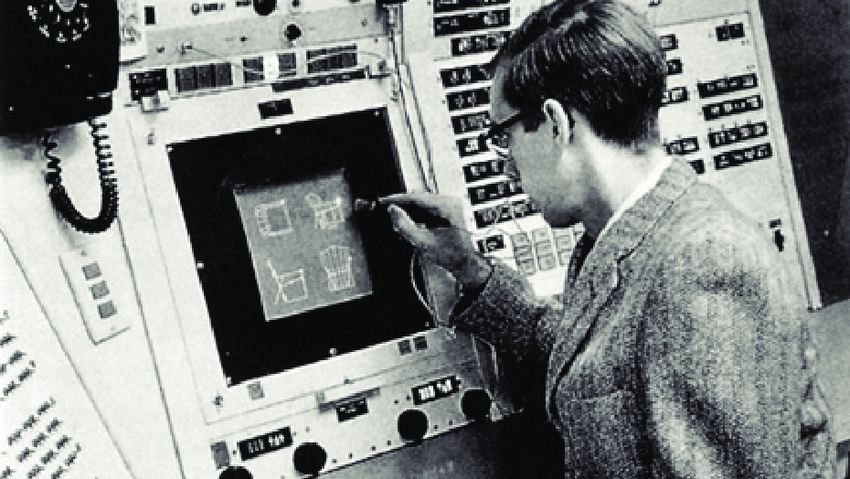
\includegraphics[width=0.7\textwidth]{sketchpad}
    \caption[Sketchpad]{Sketchpad~\cite{pic:sketchpad}}
\end{figure}

\section{Společnost \emph{Evans \& Sutherland}}
Nově vzniklá společnost měla za cíl vyvíjet počítačové simulace; zabývala se jak speciálním hardwarem pro tento účel, tak samozřejmě i softwarem. Pracovali v ní univerzitní studenti, z nichž některé inspirovala k velkým projektům. Vznikla např. společnost \emph{Adobe} Johna Warnocka (zprvu byl jejím cílem vývoj aplikací pro tisk) nebo \emph{Silicon Graphics} Jima Clarka (zabývající se hardwarem a softwarem právě pro 3D grafické aplikace)~\cite{es:birth-of-cgi}. Simulace od \emph{Evans \& Sutherland} byly používány americkou armádou a společnost existuje dodnes.

\section{Další projektování}
Tentýž rok, kdy vznikl \emph{Sketchpad}, byl také společnostmi \emph{IBM} a \emph{General Motors} k podobnému účelu vyvinut speciální počítač \emph{DAC-1}. \emph{General Motors} (americká automobilka pokrývající v tu dobu přibližně 40 \% tamějších prodejů aut~\cite{britannica:gm}) pomocí něj zrychlila projektování svých produktů~\cite{ufo:history}.

\chapter{Pokročilejší techniky -- 70.~léta}
V 70. letech byly počítače mnohem dokonalejší a dostupnější než dříve, a tak se software s 3D grafikou více rozšířil. Pořád však šlo hlavně o CAD (jsme ještě deset let před první 3D videohrou). Obecně ale grafika značně postoupila, protože byly vynalezeny nové algoritmy pro stínování\footnote{Stínování (shading) je proces, který u objektu počítá, jaké barvy modely ve scéně mají (určuje, jak reagují na světlo)~\cite{scratchapixel:shading}. Překlad stínování může být matoucí, protože záleží na chování světla při dopadu na povrch, a nikoliv na tom, jak objekty vrhají stíny.} -- Gouraudovo a Phongovo. 

\section{Gouraudovo a Phongovo stínování}
Do té doby bylo vždy používáno tzv. ploché stínování\footnote{Ploché stínování je vypočítáno pomocí normálového vektoru stěny a vektoru od světla ke stěně.} (flat shading), u něhož má celá stěna stejnou barvu. Gouraudovo i Phongovo stínování má za cíl na stěně ukázat i odlesk světla, který dodá zobrazovanému tělesu na realističnosti. Odlesk je spočítán pomocí normálového vektoru bodu odrazu, vektoru světla k bodu odrazu a vektoru od pozorovatele k bodu odrazu~\cite{javatpoint:gouraud}. Gouraudovo stínování počítá normálový vektor pro každý vrchol stěny, zatímco Phongovo stínování spočítá tento vektor pro každý pixel~\cite{javatpoint:phong}. Gouraudovo stínování je výpočetně mnohem snazší, ale vede k nepřirozenému odlesku (zejména pokud jsou stěny rozměrnější).

\begin{figure}[h]
    \centering
    \subfloat[\centering Gouraudovo stínování]{{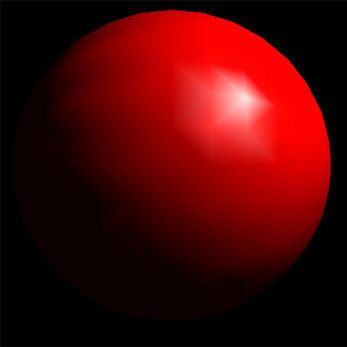
\includegraphics[width=0.35\textwidth]{gouraud}}}
    \qquad
    \subfloat[\centering Phongovo stínování]{{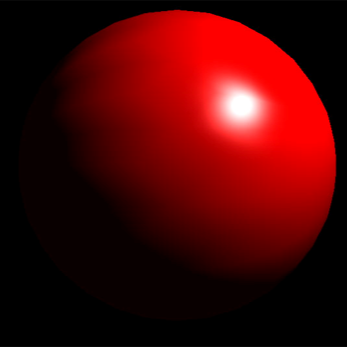
\includegraphics[width=0.35\textwidth]{phong}}}
    \caption[Druhy stínování]{Druhy stínování~\cite{pic:gouraudphong}}
\end{figure}

\section{\label{z-buffering}Z-buffering}
V roce 1974 vyvinul Wolfgang Strasser algoritmus zvaný \mbox{Z-buffering~\cite{ieee:strasser}}~-- od pozorovatele je ke všem povrchům vždy změřen vektor. Pokud je tento vektor delší než nejbližší vektor stejným směrem, pak se daný bod povrchu nevyrenderuje. Od pozorovatele je při renderování uloženo, jak daleko jsou všechny povrchy. U každého vykresleného povrchu je pak zjištěna délka vektoru od pozorovatele k němu -- tato délka se pak porovná s délkou světla k povrchu, na který dopadá v tomtéž směru. Z-buffering má za cíl zajistit, aby byly vykresleny jen ty objekty, které může pozorovatel vidět~\cite{comphope:z-buffering}.

\section{Textury}
Dobrým způsobem, jak přidat modelům v 3D grafice detail, který ve skutečnosti nemají, je textura (texture mapping); jedná se o obrázek \uvoz{nalepený} na stěnu modelu. Na obrázku může být mnohem více malých detailů, které počítač nemusí zvlášť propočítávat. Také to umožňuje snáze zobrazit materiály, na které jsme zvyklí z reálného světa. Algoritmus, který na objekt \uvoz{nalepí} texturu, vymyslel Edwin Catmull a v roce 1974 ho publikoval ve své dizertační práci (na univerzitě v Utahu). Práce algoritmu spočívá v tom, že musí více stran modelu \uvoz{polepit} stejnou texturou a ještě ji deformovat, pokud se pozorovatel nedívá na stěnu úplně kolmo~\cite{utexas:texture-mapping}.

\begin{figure}[h]
    \centering
    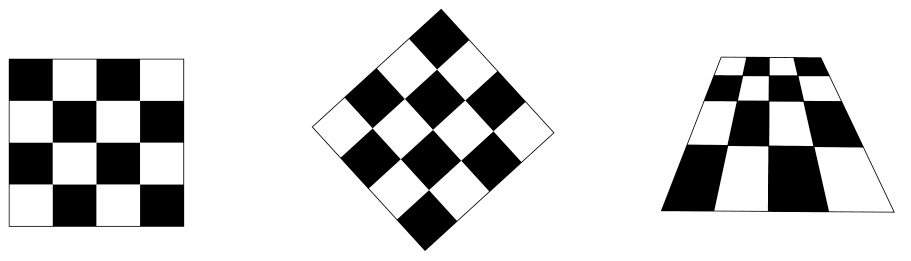
\includegraphics[width=0.85\textwidth]{texture-mapping}
    \caption[Texture mapping]{Texture mapping~\cite{utexas:texture-mapping}}
\end{figure}

\section{Stíny}
Pro další zdokonalení realističnosti scény vymyslel v roce 1978 Lance Williams shadow mapping (dva roky po dokončení studia na univerzitě v Utahu)~\cite{nvidia:shadow-mapping} -- upravení barvy textur, aby byl simulován stín, jejž objekty vrhají. Pokud je kontrolovaný povrch dále, je v tom místě textura ztmavena. Jedná se tedy o další využití Z-buffering algoritmu, který je však počítán od světelného zdroje, nikoliv od pozorovatele~\cite{wiki:shadow-mapping}.

\begin{figure}[H]
    \centering
    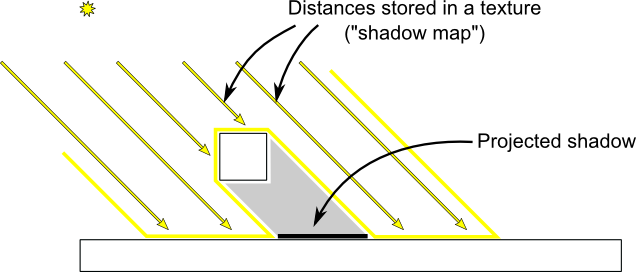
\includegraphics[width=0.85\textwidth]{shadow-mapping}
    \caption[Shadow mapping]{Shadow mapping~\cite{pic:shadow-mapping}}
\end{figure}

\section{Utažská konvička}
Pravděpodobně nejslavnější 3D model v historii vytvořil pro testovací účely v roce 1975 Martin Newell~\cite{historyoi:teapot}. Tímto modelem byla konvička z čajové soupravy, která je ale proti své reálné předloze o čtvrtinu zploštělá. Konvička byla zvolena, protože je oblá, dutá a může vrhat stín sama na sebe. Newellovu konvičku začalo používat více týmů vývojářů, protože autor 3D modelu ho zdarma zpřístupnil. Všichni potřebovali model s podobnými vlastnostmi a vytvořit jakýkoliv objekt bylo v té době poměrně složité -- souřadnice musely být vymyšleny přímo a ještě neexistoval žádný program, který by tuto činnost výrazně usnadnil.

\begin{figure}[H]
    \centering
    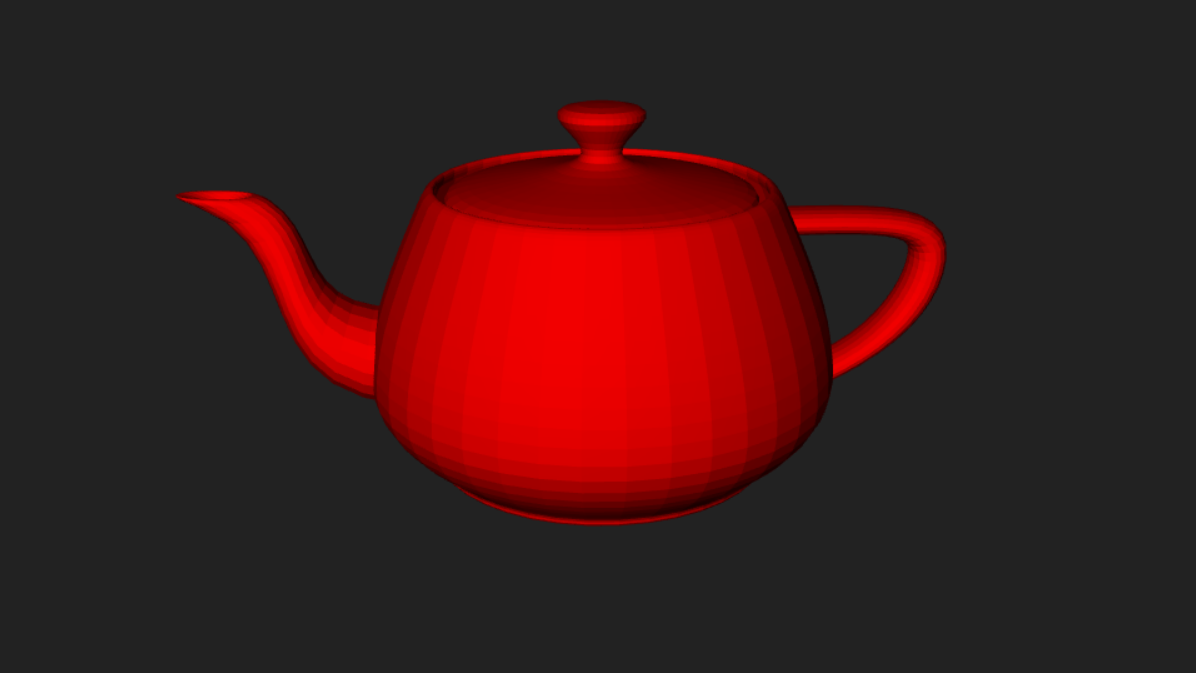
\includegraphics[width=0.75\textwidth]{teapot}
    \caption{Utažská čajová konvička}
\end{figure}
\pagebreak
\chapter{Rozšíření trojrozměrné grafiky -- 80. léta}
\section{První trojrozměrná videohra}
V 80. letech vznikly trojrozměrné videohry -- první se jmenovala \emph{Battlezone} a vyšla už roku 1980 (šlo původně o automat; později byla převedena i na herní konzole a domácí počítače). I když byly pokročilé renderovací techniky jako shadow mapping vymyšleny už o několik let dříve, trvalo ještě nějakou dobu, než byl běžný hardware schopný používat je v reálném čase. Není proto divu, že \emph{Battlezone} měl grafiku složenou jen z obrysů a bez barev~\cite{gamewiki:battlezone}.

\begin{figure}[H]
    \centering
    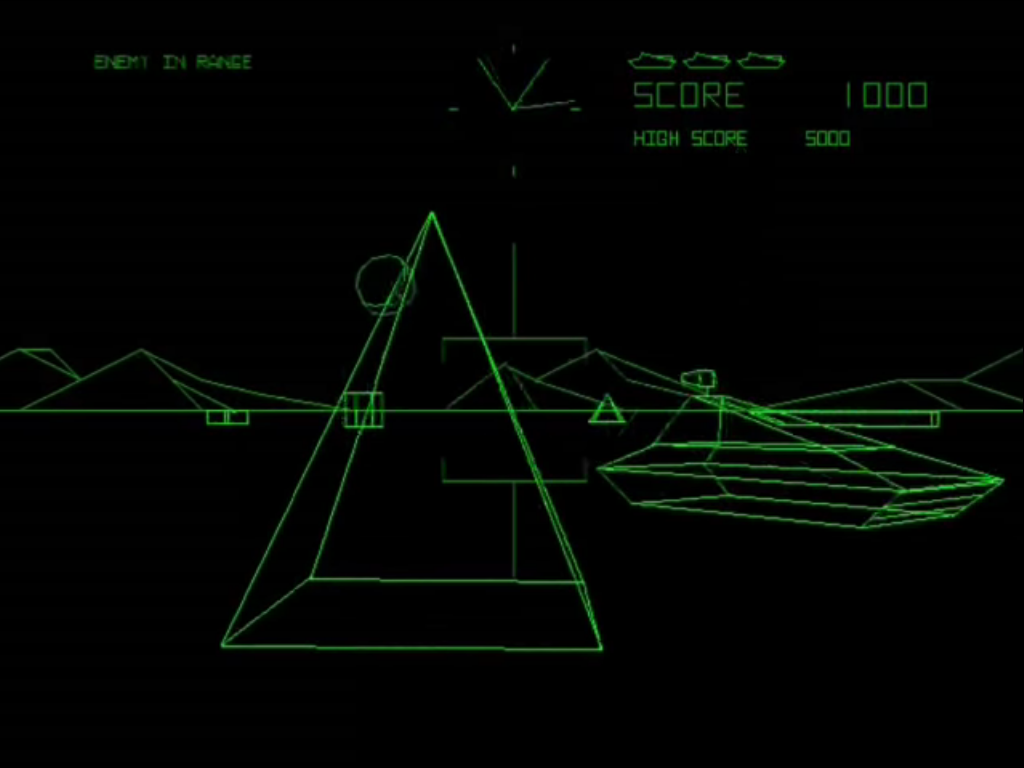
\includegraphics[width=0.7\textwidth]{battlezone}
    \caption[Battlezone (1980)]{Battlezone (1980)~\cite{pic:battlezone}}
\end{figure}

\section{Rozvoj 3D videoher}
Další zlomovou videohrou se stala \uvoz{střílečka} \emph{Driller} z roku 1987. Šlo o první hru, která by se dala označit za FPS (first person shooter -- \uvoz{střílečka} z první osoby), protože nabízela kameru otočnou do všech stran a hráč se ve hře pohyboval a střílel, jako by ve scéně stál sám~\cite{wiki:driller}. FPS je dnes jedním z nejrozšířenějších videoherních žánrů a je zcela založen na 3D grafice. Hlavním příčinou úspěchu této videohry byla její technická pokročilost umožněná 3D enginem\footnote{Engine je software, který uživateli (v případě 3D enginů jde většinou o herní vývojáře nebo animátory) umožňuje snazší komunikaci s hardwarem a softwarem pro renderování scény; jeho součástí také často bývá např. fyzika napodobující reálný svět~\cite{techjunkie:engine}.} \emph{Freescape}, který byl později použit ještě v několika dalších hrách. Zásadní rozdíl v grafice her \emph{Battlezone} a \emph{Driller} představovaly (kromě kamery) vyplněné stěny objektů ve scéně; nejednalo se už jen o obrysy. Stále ale bylo vše bez textur a bez osvětlení, jen s velmi malým rozlišením.

\begin{figure}[H]
    \centering
    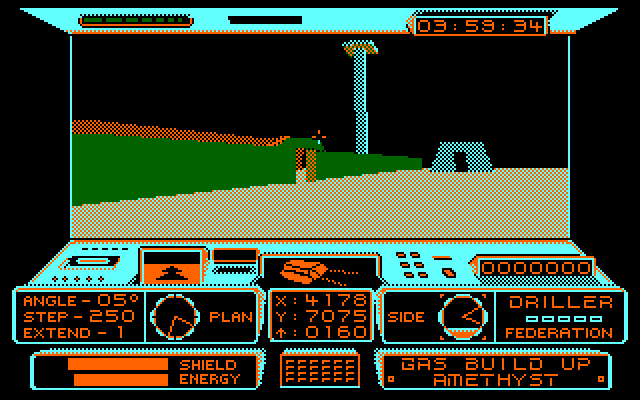
\includegraphics[width=0.75\textwidth]{driller}
    \caption[Driller (1987)]{Battlezone (1987)~\cite{pic:driller}}
\end{figure}

\section{Profesionální modelování}
Obecně se 3D grafika dostala do rukou daleko většího množství uživatelů než dříve, protože se v roce 1981 začal sériově vyrábět první \emph{Osobní počítač IBM} (zkratka IBM PC) s rekordními prodeji pro svoji relativně nízkou cenu~\cite{ibm:pc}. Pro rychlejší vytváření prototypů z mnohem rozšířenějšího softwaru CAD byl vynalezen 3D tisk (i když první zařízení, které koncept v praxi využilo, bylo vyrobeno až roku 1992~\cite{bcn3d:invention}). Dvojrozměrný \emph{AutoCAD} byl mnohem levnější než jakýkoliv dřívější program na projektování, navíc byl vyvinutý pro IBM PC~\cite{cadstudio:history}. K projektování modelů na počítači začali v tuto dobu přecházet od tužky a papíru i architekti.

\chapter{Zdokonalení -- 90. léta}
\section{Textury ve videohrách}
V 90. letech se již objevily první videohry s texturami. Hardware v tu dobu ale pořád zdaleka nebyl natolik silný, aby trojrozměrně v reálném čase zobrazoval vše, co je na scéně. Proto se přistoupilo ke kombinaci, kde prostředí, v němž se hráč pohyboval, bylo složeno z uzavřených jednoduchých trojrozměrných místností. Všechno ostatní byly dvojrozměrné sprity\footnote{Sprite je ve videohře dvojrozměrný obrázek předmětu nebo jeho části -- pohyb je vyjádřen manipulací se sprity; většinou jsou animované.}. Když hráč chodil v místnosti okolo předmětů nebo nepřátel, jejich sprity se pořád otáčely za ním. Této technice kombinace 2D a 3D grafiky se někdy říkalo 2,5D a první hrou, která ji použila, byl \emph{Wolfenstein 3D} z roku 1992~\cite{techradar:evolution}.

\begin{figure}[h]
    \centering
    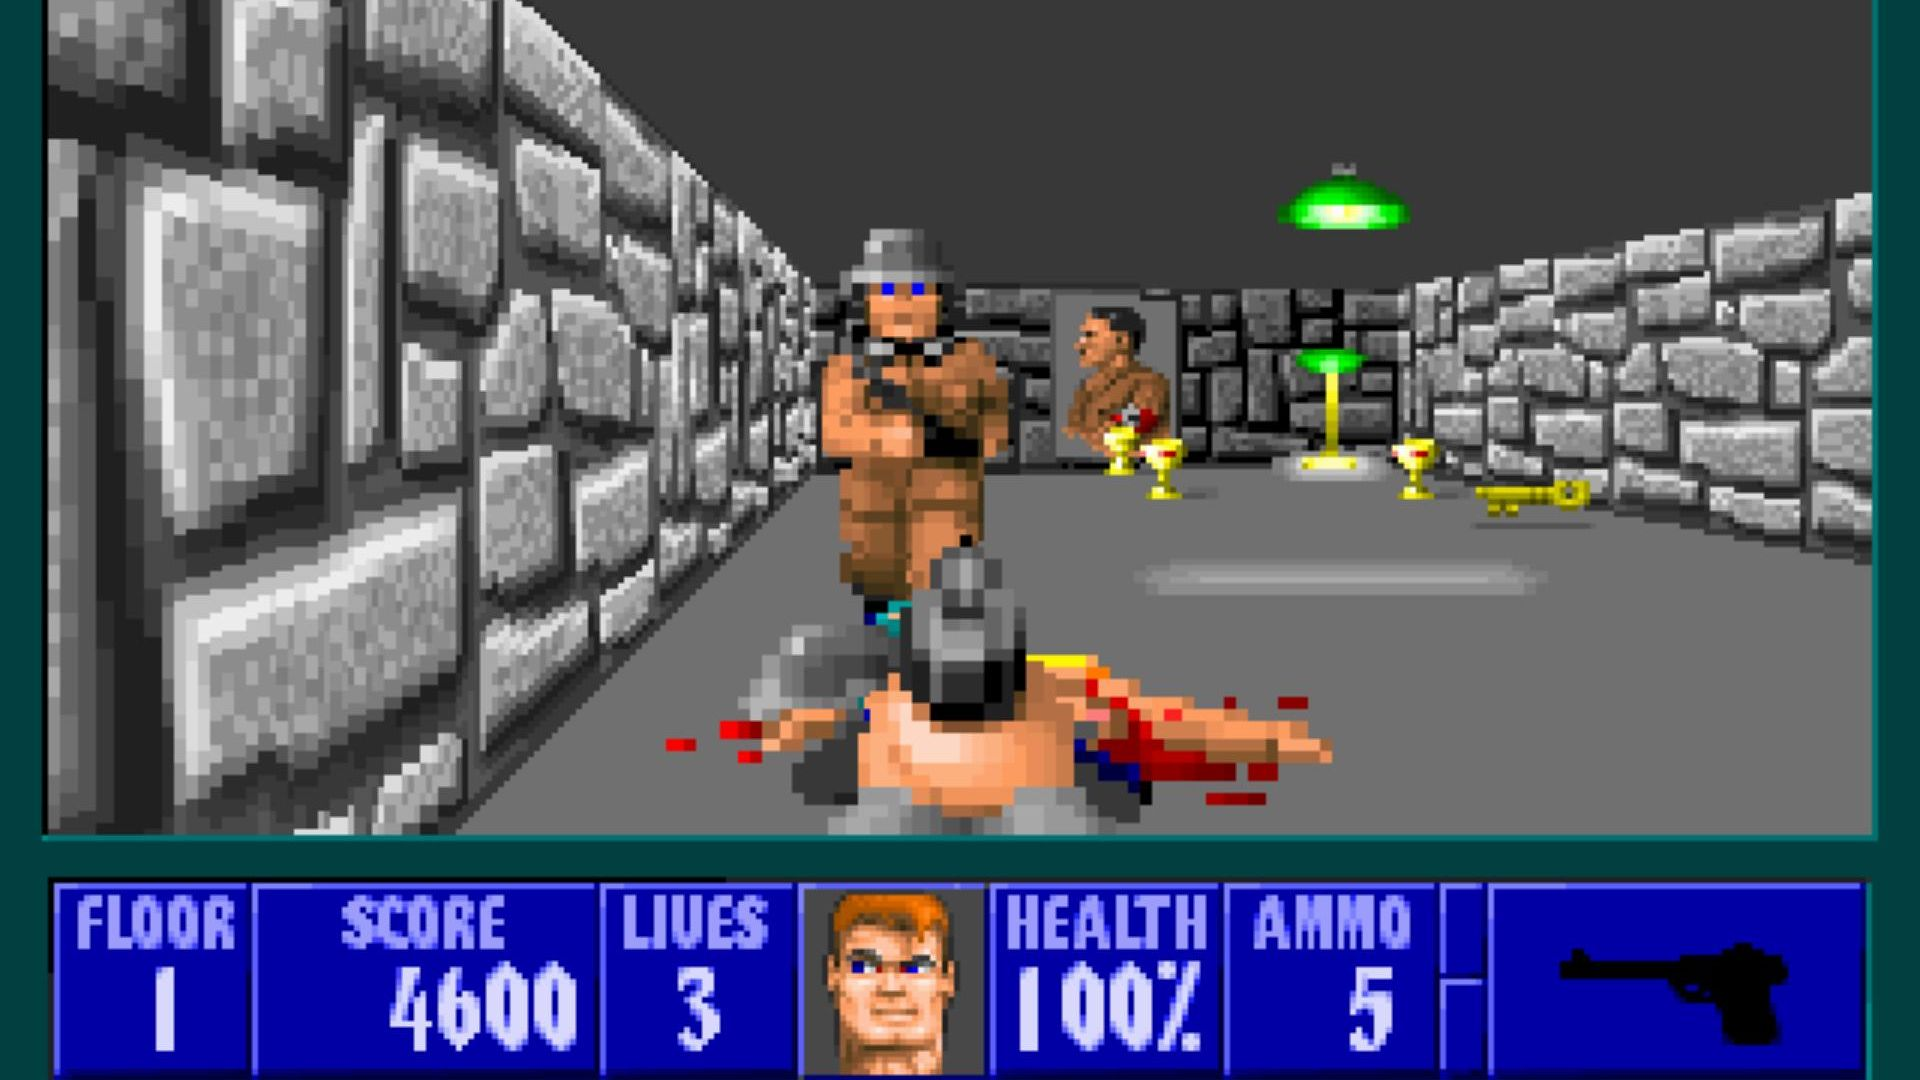
\includegraphics[width=0.75\textwidth]{wolfenstein}
    \caption[Wolfenstein 3D (1992)]{Wolfenstein 3D (1992)~\cite{pic:wolfenstein}}
\end{figure}

\section{Limity 2,5D}
Ačkoliv se jednalo o na první pohled velmi pokročilou techniku, měla značné limity. Oproti hrám s enginem \emph{Freescape} běželo vše mnohem plynuleji, ale na druhou stranu se ztratila volně otočná kamera. Iluze předmětů v prostoru jen pomocí 2D spritů mizela, pokud bylo hráči umožněno kamerou točit směrem nahoru a dolů (u většiny herních titulů byla proto tato možnost odstraněna). Také všechny mapy byly pořád dvojrozměrné; v jednu chvíli nebylo možné renderovat místnosti nad sebou (používaly se různé triky na zamaskování tohoto nedostatku, např. skryté teleporty do nových místností)~\cite{techradar:evolution}.

\section{Překonání 2,5D}
Nejprve byly do kompletního 3D (vše bylo renderováno v trojrozměrném prostoru s texturami) přeneseny jednodušší žánry na zpracování. Roku 1992 byl vydán \emph{Virtua Racing}. První hrou, která opravdu překonala předchozí 2,5D, se stal \emph{Quake} (vydaný v roce 1996)~\cite{pcmag:history}. V této \uvoz{střílečce} se také hojně vertikálních možností herní mapy využívalo. Nepřátelé neměli tak kvalitní textury, jako byly dřívější sprity, ale vypadali \uvoz{jako opravdoví}. S plně trojrozměrnými hrami se také na trhu objevily první grafické karty specializované na renderování 3D grafiky~\cite{newegg:gpu}.

\begin{figure}[h]
    \centering
    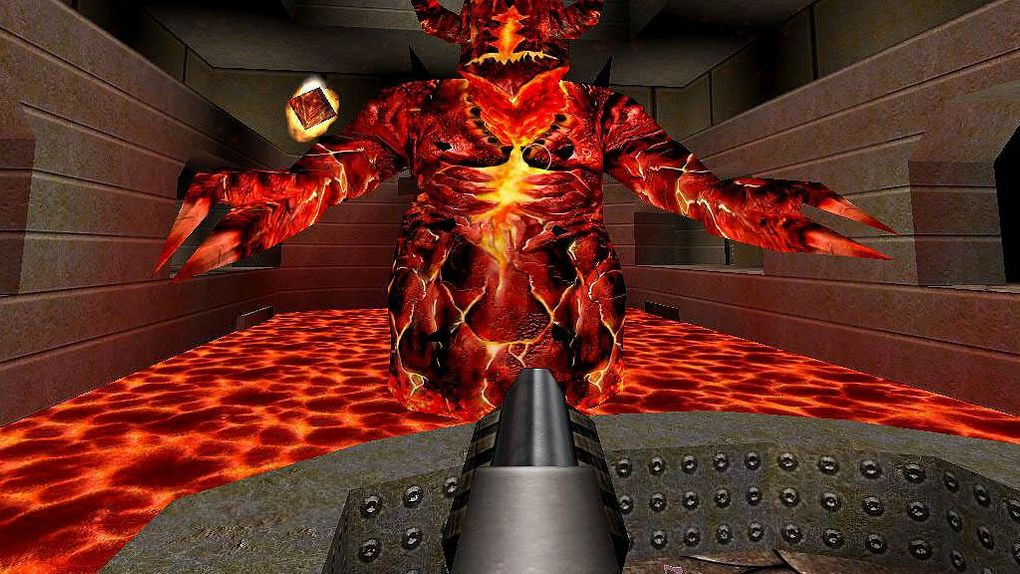
\includegraphics[width=0.75\textwidth]{quake}
    \caption[Quake (1996)]{Quake (1996)~\cite{pic:quake}}
\end{figure}

\section{Software pro modelování}
V 90. letech také vznikla velká část programů, které se pro vytváření trojrozměrných modelů používají dodnes. Samozřejmě od té doby prošly výraznými změnami, ale právě kvůli takto dlouhému vývoji je velmi těžké se jim dnes vyrovnat. Mezi ně patří např. \emph{Cinema 4D}, \emph{Blender} nebo \emph{3D Studio MAX}. V té době se k softwaru pro modelování 3D grafiky mohl dostat každý, kdo měl dostatečně silný počítač -- \emph{Blender} je otevřený software.

\chapter{Současnost}
Po roce 2000 v samotné technice zobrazení k výrazným změnám nedošlo. Na druhou stranu se ve velkém měřítku zdokonalilo vše, co do té doby existovalo. Např. virtuální realita, která v dřívějších dobách byla možná spíše jen teoreticky, se dnes stává skutečností. První pokus o běžně dostupnou virtuální realitu představovala konzole \emph{Virtual boy} už z roku 1995~\cite{nintendowiki:virtualboy}. Hardware z té doby nebyl pro realistické zobrazení dostatečně silný. I dnes, kdy je rozlišení několikanásobně větší než v té době, ještě stále není dostatečné. K většině zlepšení dochází kvůli silnějšímu hardwaru a optimalizaci softwaru. Díky nim je možné použít detailnější textury a komplikovanější modely. I když je tvořena animace, která nemusí běžet v reálném čase, je vždy potřeba mít k dispozici dostatečně silný hardware, aby se s modely ve scéně dalo na počítači manipulovat alespoň po částech.

\begin{figure}[H]
    \centering
    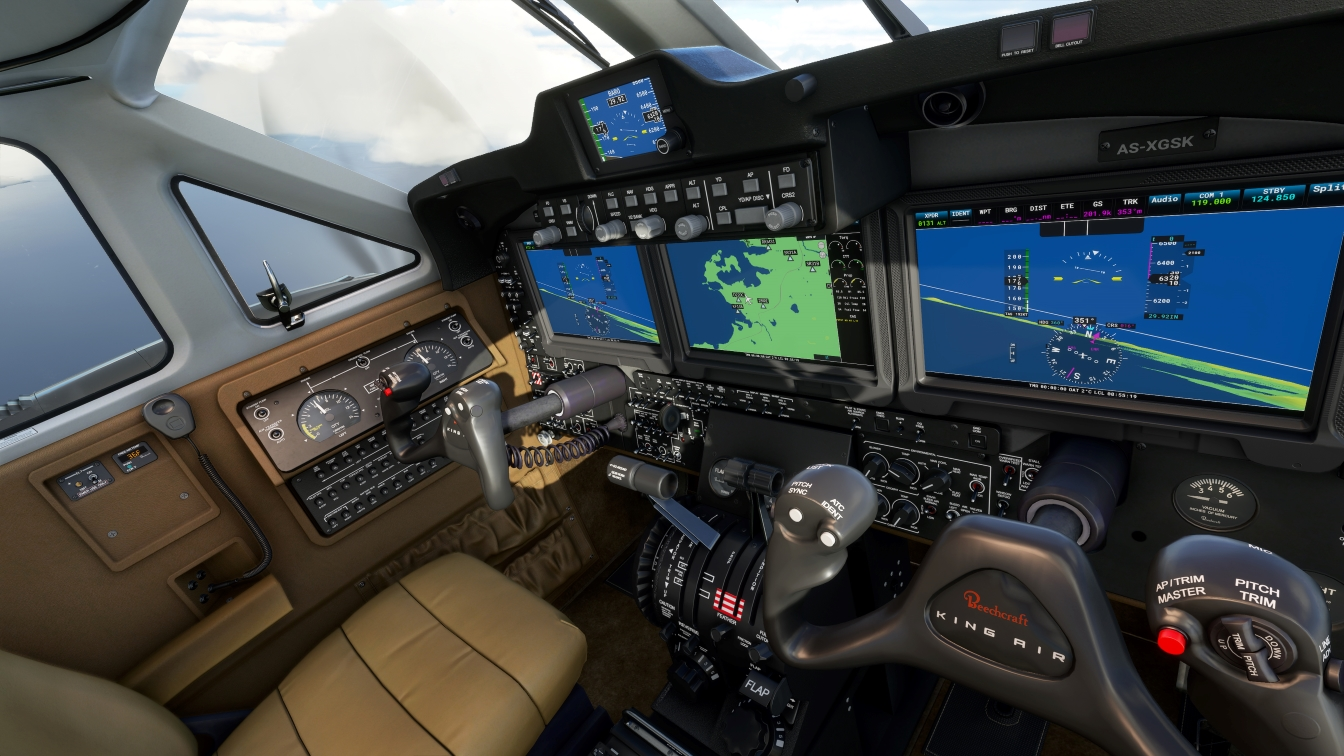
\includegraphics[width=0.8\textwidth]{msflightsim}
    \caption[Microsoft Flight Simulator (2020)]{Microsoft Flight Simulator (2020)~\cite{pic:msflightsim}}
\end{figure}

\end{chapterwithoutpagebreak}
\part{Praktická část}
\chapter{Cíle práce}
Cílem práce bylo naprogramovat aplikaci, jež by umožňovala uživateli nahrát soubory typu Wavefront object (formát vyvinutý americkou společností Wavefront pro jejich program Advanced Visualizer~\cite{wiki:obj}; později byl tento formát přijat ostatními společnostmi a je považován za standard). Na toto načtení jsem se rozhodl použít pouze standardní knihovny C++ a algoritmy na syntaktickou analýzu souboru či triangulaci si napsat sám (nebo v případě triangulace sám napsat implementaci již vymyšleného algoritmu). Kromě nahrání souboru by měl mít uživatel možnost prohlížet si objekty jím ovládanou kamerou a aranžovat je do scén, tedy posouvat jimi, otáčet je, měnit jejich velikost.

Protože vytvoření 3D editoru se všemi funkcemi je projekt úplně jiného měřítka než maturitní práce, navíc je na trhu mnoho možností včetně projektů otevřeného softwaru (např. Blender), bylo cílem hlavně si vyzkoušet práci s knihovnami, které by byly pravděpodobně použity při vývoji takové aplikace. Pro prostorové zobrazování jsem se chtěl vyhnout enginům, které právě zprostředkují vývojářům snazší komunikaci s nízkoúrovňovými grafickými knihovnami. Kromě prostorového zobrazení bylo cílem vytvořit uživatelské prostředí s nativním ovládáním operačního systému, protože prvky nakreslené pomocí API operačního systému jsou více flexibilní a vypadají lépe než ta, jež bych kreslil sám. Například systémová tlačítka už mají animaci a také mezi nimi lze přeskakovat pomocí šipek.

\chapter{Způsoby řešení a použité postupy}
Program je rozdělen do více souborů a tříd, aby se v něm dalo lépe orientovat. Konkrétně se jedná o pět souborů hlaviček s definicemi tříd, pět souborů s implementacemi těchto tříd a dva soubory shaderů pro knihovnu OpenGL. Základ programu leží v souborech \emph{main.hpp} a \emph{main.cpp}.

Všechny třídy v těchto souborech jsou zděděny z tříd knihovny wxWidgets, protože zprostředkují grafické prostředí. Okna jsou zděděna ze třídy \texttt{wxFrame}. Ta samotná většinou k uspokojivému rozložení ovládacích prvků nestačí, proto se do oken vkládají tzv. panely (ze třídy \texttt{wxPanel}). Rozložení panelů nebo samotných ovládacích prvků je určeno kontejnery ze třídy \texttt{wxSizer}; mají za úkol měnit velikost a polohu obsažených prvků podle místa, jež mají k dispozici. Tyto kontejnery umožňují určit, kolik místa mohou tlačítka, textová pole nebo panely v nich zabírat.

Protože aplikace vytvořená pomocí knihovny wxWidgets je řízená událostmi (eventy), musíme u tříd, kde o to máme zájem, nastavit tabulku zachytávání událostí. V ní pomocí maker stanovíme, jaká funkce se má při dané události spustit. Tato tabulka musí být v hlavičce nejprve deklarována uvnitř každé třídy, kde chceme události zachytávat, a potom zvlášť definována (zde v kódu vždy nad příslušnou třídou).

WxWidgets v sobě obsahuje velké množství tříd, které mají přímý ekvivalent ve standardní knihovně. Jako příklad můžeme uvést textové řetězce (\texttt{string}), vzájemné vyloučení (\texttt{mutex}), vlákna (\texttt{thread}), kontejnery vektor (\texttt{vector}); je jich relativně velké množství. Třídy z wxWidgets a jejich metody používají ve svých argumentech nebo návratových hodnotách právě tyto jiné verze už standardně implementovaných kontejnerů či tříd. Ze standardních datových typů (nebo zpět na ně) je nutné je převést a tento převod není vždy implicitní. V projektu jsem se snažil oddělit části kódu s knihovnou wxWidgets od ostatního kódu; nestandardní datové typy a třídy (z wxWidgets) se snažím nepoužívat mimo třídy zděděné z wxWidgets a soubory \emph{main.hpp} a \emph{main.cpp}.

Při práci jsem používal dokumentaci programovacího jazyka C++\footnote{\url{https://en.cppreference.com/w/}} a knihoven: wxWidgets\footnote{\url{https://docs.wxwidgets.org/3.1/}}, GLM\footnote{\url{https://glm.g-truc.net/0.9.9/api/index.html}} a OpenGL\footnote{\url{https://docs.gl/}}. U informací, které jsem se dozvěděl z dokumentace, je explicitně jako zdroje neuvádím.

Podle dvou zdrojů jsem se v některých částech orientoval, protože jsem nikdy podobný projekt nedělal. Těmito zdroji jsou: tutoriál OpenGL\footnote{\url{https://learnopengl.com/}} a ukázkový projekt \emph{Pyramid} od wxWidgets\footnote{\url{https://github.com/wxWidgets/wxWidgets/tree/master/samples/opengl/pyramid}}. Pomohly mi obecně s použitím vertex array; výpočtem umístění bodů (využití příslušných transformačních matic) ve scéně; OpenGL plátnem a kontextem ve wxWidgets. Jen pomocí dokumentace jsem mohl obtížně poznat, jaké funkce nebo části potřebuji využít. Dokumentace mi byla užitečná až v době, kdy jsem alespoň přibližně věděl, co chci použít (poradila mi, jak se vybrané části používají, popř. mi pomohla najít vhodnější alternativu). Pokud jsem nějakou část kódu okopíroval, umístil jsem k ní (do zdrojového kódu) komentář se zdrojem (jedná se např. o výpočet barvy v fragment shaderu nebo výpočet průměrné frekvence zobrazení).

\section{Třída \texttt{App}}
Tato třída se dá považovat za úplný základ aplikace, je zděděná z třídy \texttt{wxApp} a kromě předefinování virtuální funkce \texttt{OnInit} se od své rodičovské třídy nijak neliší. Hlavní smyčka programu je součástí této třídy a většinou ji při vývoji aplikace s knihovnou wxWidgets není nutné předefinovat, protože jednotlivé funkce programu jsou spouštěny pomocí událostí; implementace nových částí programu až na výjimečné případy změnu hlavní smyčky nevyžaduje.

Funkce \texttt{OnInit} připraví příslušné části wxWidgets na načítání obrázků textur a spustí hlavní okno aplikace. Pokud se toto okno úspěšně spustí včetně plátna (canvas) na vykreslování scény (to se ověří funkcí \texttt{openGLInitialized} patřící třídě hlavního okna), vrátí funkce hodnotu \emph{true} (pravda) a hlavní smyčka se spustí. V opačném případě je zobrazena uživateli chybová hláška a aplikace posléze uzavřena.

\section{Hlavní okno -- třída \texttt{MainFrame}}
Nejdůležitější viditelnou částí programu (se kterou také uživatel bude nejčastěji interagovat) je hlavní okno. Z něj jsou později otevírána všechna ostatní okna a zároveň je jeho součástí většina ovládacích prvků.

V konstruktoru třídy hlavního okna je načtena ikona programu~\cite{pic:icon}, vytvořena nabídka v levém horním rohu a stavový řádek, jenž bude později použit pro zobrazení počtu vykreslených snímků za vteřinu. Uvnitř konstruktoru je také ověřeno, že OpenGL půjde spustit. Pokud ano, je vytvořeno plátno pro OpenGL a postranní panel s ovládáním objektů.

\section{Postranní panel -- třída \texttt{SidePanel}}
Třída postranního panelu má za úkol držet v sobě třídy umožňující uživateli interakci s objekty. Těmi třídami jsou \texttt{ObjectList}, \texttt{ObjectSettings} a \texttt{SidePanelRefreshTimer}. První dvě z jmenovaných tříd jsou panely a zbývající je třída časovače (zděděná z \texttt{wxTimer}).

Všechna nastavení v postranním panelu mění parametry objektů podobným způsobem. Při stisknutí tlačítka nebo úpravě nastavení je provedena kontrola, zda je nějaký objekt zvolen. Pokud zvolen není, tlačítka nemají žádný účinek (ani se nezobrazí menu možnosti změny textury nebo jména) a číselná pole s roletou se vrací do své původní (nulové) polohy. Pokud cílový objekt zvolen je, pak je změna přeposlána do třídy \texttt{GraphicsManager}, která drží všechny objekty.

\subsection{Třída \texttt{ObjectSettings}}
Tato třída má za úkol spravovat číselná pole (se souřadnicemi objektů, jejich rotací, velikostí) a roletu s výběrem renderovacího režimu stěn. \texttt{ObjectList} v sobě drží tlačítka pro manipulaci s objekty a seznam třídy \texttt{wxCheckListBox}, ve kterém si uživatel může vybírat objekt, jejž chce upravit nebo s ním manipulovat. Při interakci s tlačítky nebo poli v postranním panelu si funkce zachycující událost (stisknutí nebo změny hodnoty uvnitř pole) z listu zjistí, který objekt chce uživatel upravovat. Další úlohou seznamu je také ukazování a schovávání objektů na scéně.

\subsection{Třída \texttt{SidePanelRefreshTimer}}
Cílem časovače je držet uživatelské rozhraní aktuální, tedy v souladu se skutečným stavem objektů. Virtuální metoda \texttt{Notify} se periodicky spouští; v každém cyklu je zkontrolován seznam, zda se v něm něco nezměnilo (v případě změny je seznam upraven), a také je aktivována událost třídy \texttt{ObjectSettings}, aby se analogicky zkontrolovala i číselná pole a roleta.

\section{Plátno -- třída \texttt{Canvas}}
\subsection{Co je plátno?}
Abychom mohli vidět, co OpenGL vykreslí, je nutné mít třídu zděděnou z \texttt{wxGLCanvas}, která bude s OpenGL komunikovat -- plátno je místo, do kterého se mohou vkládat tzv. kontexty (v knihovně wxWidgets jsou kontexty implementovány třídou \texttt{wxGLContext}). Kontexty zařizují celkovou komunikaci s OpenGL; nejen obraz, ale i všechna volání. Kontext drží v každém okamžiku dva snímky v tzv. bufferech; jeden je ukazován uživateli a na druhém pracuje OpenGL. Když je snímek na pozadí kompletně vykreslen, můžou být buffery vzájemně vyměněny; uživatel pak vidí nový snímek a OpenGL mezitím vykresluje nový.

Třída \texttt{Canvas} má několik rolí. Nejdůležitější je pravidelné zobrazování vykreslených snímků uživateli (v průběhu ještě počítá průměrnou obnovovací frekvenci, kterou zapisuje do stavové lišty v levém spodním rohu okna). Další rolí je monitorování akcí uživatele (pohyb myší, stisknutí tlačítek myši) a změna velikosti viewportu (průzoru, do něhož OpenGL renderuje) podle aktuální velikosti okna.

V konstruktoru této třídy se vytvoří nový kontext a je zkontrolován, zda běží správně. Pokud se kontext řádně vytvořil, inicializuje se knihovna GLEW, jež načte grafickou kartou (o ovladačem) podporovaná rozšíření (extensions) OpenGL. GLEW také nastaví potřebné konstanty a ukazatele (pointers) na funkce OpenGL. Než může program začít vykreslovat, je ještě potřeba zkontrolovat dostupnost všech rozšíření, s nimiž budeme později pracovat. K tomu slouží funkce \texttt{extCheck}, se kterou jsou všechna potřebná rozšíření otestována. Pak už zbývá jen vytvořit třídu \texttt{GraphicsManager} a spustit renderovací smyčku.

\subsection{Renderovací smyčka}
Během řešení problému renderovací smyčky se ukázalo, že wxWidgets možná není nejlepší knihovnou pro tento úkol, protože její nejlepší stránka není v rychlosti hlavní smyčky a optimalizaci, ale v jednoduchosti používání grafických prvků. WxWidgets má pro tento účel velký výběr možností, ale téměř žádný pro snadné vytvoření renderovací smyčky. Návod k wxWidgets radí, aby byl použit časovač (stejně jako je vyřešen časovač na aktualizování seznamu objektů a nastavení)~\cite{wx:render}. Tento přístup má značnou nevýhodu -- časovače wxWidgets používají tzv. low precision (málo přesný) časovač operačního systému. To by nebyl problém na jiné platformě, než je operační systém Windows. Ale právě tady je časovač opravdu relativně nepřesný; skáče přibližně po 15--16 ms~\cite{ms:timer}, a hlavně se nedokáže spouštět okamžitě -- s nulovou dobou čekání (což by bylo ideální). S takovou minimální dobou dosáhne aplikace obnovovací frekvence scény přibližně 60 Hz. To by u většiny počítačů nepředstavovalo žádné omezení, protože monitory s obnovovací frekvencí 60 Hz patří pořád k nejběžnějším.

Já jsem ale chtěl, aby aplikace nebyla v tomto ohledu limitována, protože monitory s vyšší obnovovací frekvencí jsou čím dál častější a nová aplikace by na to měla být připravena. Proto jsem přistoupil k řešení, od něhož návod zrazuje. Po připravení okna a plátna s kontextem je spuštěna renderovací událost, která vykresluje, opakovaně spouští sama sebe a volá metodu \texttt{Yield} třídy \texttt{App}. Volání této metody je nezbytné, protože aplikaci umožňuje zachycovat ostatní události; bez ní by aplikace zamrzla. V době, kdy se uživatel rozhodne aplikaci ukončit, se událost přestane volat a program se normálně uzavře. Tímto způsobem aplikace vykresluje nejvyšší rychlostí, jakou je jí to dovoleno počítačem. To také není ideální stav; je řešen v třídě \texttt{GraphicsManager} pomocí tzv. vertikální synchronizace, která upravuje obnovovací frekvenci programu podle obnovovací frekvence monitoru. Tento přístup se i přes varování v návodu ukázal jako plně funkční s výhodami oproti doporučenému.

\section{Třída \texttt{GraphicsManager}}
Tato třída má za úkol vykreslovat scénu s knihovnou OpenGL a provádět v ní všechny změny, o které uživatel zažádá přes ovládací prvky grafického rozhraní. Drží v sobě všechny objekty i textury a s použitím metod této třídy jsou upravovány jejich parametry.

\subsection{Konstruktor}
Při vytvoření třídy \texttt{GraphicsManager} je zapnuta vertikální synchronizace (zkráceně v-sync), jež má za cíl zpomalení výměny vykreslených snímků a vykreslování nových tak, aby frekvence vykreslování nepřesahovala frekvenci monitoru. Pokud to grafický ovladač (a monitor) dovoluje, zapne se v-sync v tzv. adaptivním režimu pro zmenšené trhání obrazu -- pokud vykreslený snímek netrefí frekvenci monitoru a je připraven příliš pozdě, vykreslí se ihned místo čekání na další snímek monitoru.

\begin{minipage}{\textwidth}
Dále je v OpenGL aktivován test hloubky (Z-buffering), který zařídí, že při vykreslování zůstane na vršku snímku vždy jen to, co se v prostoru nachází blíže ke kameře\footnote{Další informace o Z-bufferingu jsou v části \ref{z-buffering}.}. Bez tohoto testu by se mohlo stát, že zadní stěna zobrazeného objektu se vykreslí přes přední (obr. \ref{depthtest}).
\end{minipage}

\begin{figure}[h]
    \centering
    \subfloat[\centering Renderování bez testu hloubky]{{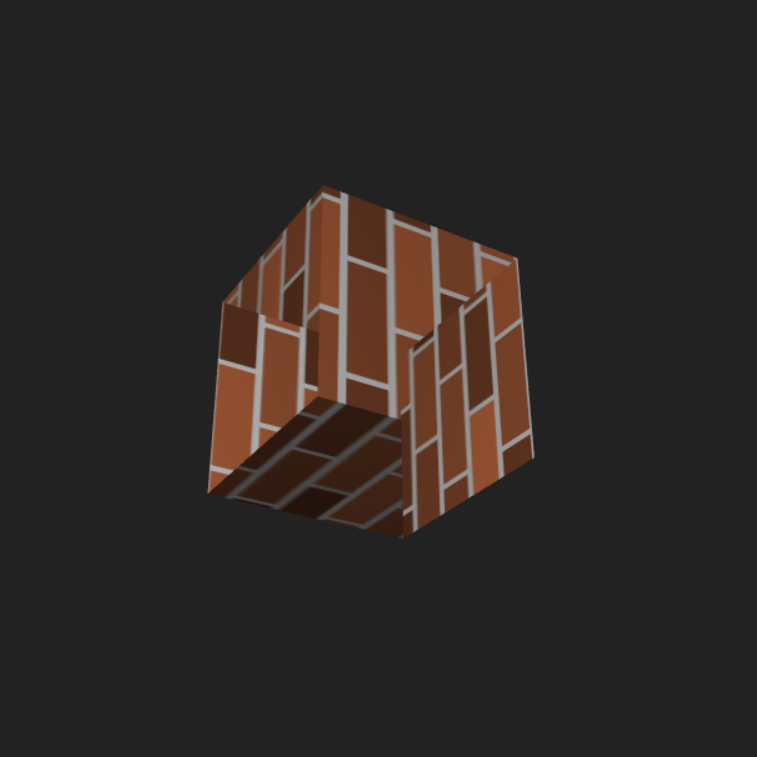
\includegraphics[width=0.45\textwidth]{without-depth-test}}}
    \qquad
    \subfloat[\centering Renderování s testem hloubky]{{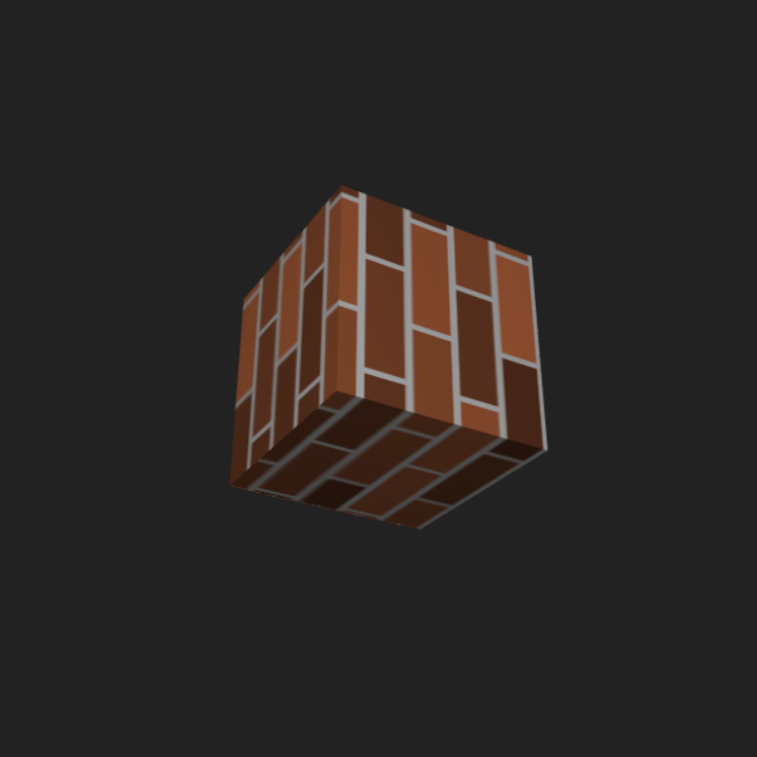
\includegraphics[width=0.45\textwidth]{with-depth-test}}}
    \caption{\label{depthtest}Test hloubky}
\end{figure}

Než může vykreslování začít, je potřeba vytvořit třídu spravující polohu a směr kamery (třída \texttt{Camera}) a načíst shadery\footnote{Bližší informace o shaderech viz \ref{shadery}} pomocí třídy \texttt{ShaderManager}. Jsou načteny ze souborů ve složce s aplikací -- \emph{default.vert} je soubor s vertex shaderem a \emph{default.frag} je soubor s fragment shaderem.

Pokud je program postaven v režimu ladění (debug), je v konstruktoru také zapnuto vypisování chyb (a informací) z OpenGL do terminálu. Pro výpis je použita funkce \texttt{GLDebugMessageCallback}, kterou jsem převzal a upravil. Sám jsem ji nevytvořil, protože jsem nevěděl, co přesně jednotlivé hodnoty znamenají. Úprava byla potřeba, protože byla tato funkce napsaná původně pro jiný kompilátor (MSVC), než používám, a protože jsem chtěl, aby zobrazovala všechny zprávy včetně informačních.

\subsection{Správa objektů a textur}
Objekty i textury jsou zvláštní třídy (třída \texttt{Object} a \texttt{Texture}), které jsou drženy v kontejnerech typu \texttt{vector}. Přesněji řečeno v těchto kontejnerech se ukládají chytré ukazatele (smart pointer) k těmto třídám. Velkou výhodou ukazatelů proti přímému ukládání objektů je, že není třeba tolik místa v kontejneru \texttt{vector}. Pokud bude třeba uložit více dat, než kolik je momentálně místa, stačí při zvětšování \texttt{vectoru} potřeba méně nového místa v heapu u sebe a kopírování všech již zapsaných dat do nového (většího) místa v paměti se mnohonásobně zrychlí. Chytré ukazatele mají oproti standardním výhodu v tom, že pokud se ocitnou mimo rozsah programu, jsou automaticky smazány, a není tedy třeba jejich data z paměti odstraňovat explicitně. Na objekty je ukazováno pomocí \texttt{unique\_ptr}, který může být vždy držen v programu jen na jednom místě; v této aplikaci je vždy držen pouze třídou \texttt{GraphicsManager} a všechny požadavky na data (ať jejich čtení nebo zápis) jsou vyřizovány přes její metody. K texturám je přistupováno s použitím ukazatele \texttt{shared\_ptr}, jenž umožňuje jeho držení na více místech zároveň (ukazatel si sám počítá, v kolika místech je stále používán; pokud už není používán nikde, smaže data, na která ukazuje). K texturám jsem zvolil raději tento typ ukazatele, protože pokud se uživatel ze seznamu rozhodne odstranit texturu, která je právě některým objektem používána, objekt o ni nepřijde; je odstraněna až v moment, kdy není ani v seznamu a ani ji nepoužívá žádný objekt. V uživatelském rozhraní jsou objekty či textury v seznamech seřazeny stejně jako uvnitř kontejnerů \texttt{vector} a pokud uživatel některou položku ze seznamu vybere, je tím zjištěn index upravovaného objektu či textury. S tímto indexem se pak zavolá metoda třídy \texttt{GraphicsManager} pro danou operaci s objektem nebo texturou.

\subsection{Načítání nového objektu}
I když na načítání objektů z různých typů souborů (včetně Wavefront object) existují knihovny, mým záměrem bylo udělat logiku načítání sám. Tato aplikace kvůli tomu není v současném stavu schopná načítat další typy souborů. Samotné načítání začíná ve funkci \texttt{newObject}, která je volána při stisknutí tlačítka \emph{New} v postranním panelu nebo při zvolení možnosti \emph{Load object...} v menu.

\subsubsection{Syntaktická analýza souboru}
Zvolený soubor je zpracován funkcí \texttt{parseFile} -- ta rozdělí celý soubor do kontejneru \texttt{vector}, v němž jsou další \texttt{vectory} (každý reprezentuje řádek v souboru). Data na každém řádku jsou mezerami rozdělena do \uvoz{bloků}; blok je samostatný řetězec znaků (\texttt{string}). Toto rozdělení je užitečné z důvodu, že tak půjde dobře dělit řádky podle prvního bloku (který určuje, jaké informace se na řádku nacházejí). Kromě toho rozdělení umožňuje snazší převod znakových řetězců s čísly na samotná čísla -- v každém bloku se nachází vždy jen jedno číslo bez jiných znaků, tudíž lze převést celý řetězec bez úprav. V kontejnerech reprezentující řádky jsou uložené jednotlivé bloky textu. Kromě jednoduchého rozdělení souboru je úkolem funkce \texttt{parseFile} přeskakování všech řádků s komentáři a spojování řádků, které končí zpětným lomítkem (\textbackslash). Dále se funkce \texttt{parseFile} umí vypořádat i s prázdnými řádky a vícero mezerami mezi bloky, které do výsledného kontejneru nezapíše.

Po rozdělení souboru jsou jednotlivé řádky čteny a data z nich zpracovávána. Vždy je přečten první blok v každém řádku a podle něho jsou následně data zpracována. Funkce \texttt{newObject} je rekurzivní, protože v souboru může být i více objektů než jen jeden. Aby se nezaplnila paměť počítače při načítání souboru s větším množstvím objektů, jsou všechna společná data sdílena mezi rekurzivními voláními (v kontejnerech) pomocí chytrých ukazatelů (zde je použit konkrétně \texttt{shared\_ptr}). Mezi společná data\footnote{Bližší informace o využití dat viz \ref{objekt}} patří soubor rozdělený do řádků a bloků, souřadnice bodů v prostoru i v obrázku textury a normálové vektory pro výpočet osvětlení objektu. Naopak každé volání \texttt{newObject} si zvlášť drží informace o bodech konkrétního objektu (v prostoru i v textuře, a navíc ještě normály), které jsou uvedeny ve specifickém pořadí pro daný objekt a mohou se i opakovat (jsou vybrány ze společných dat).

Wavefront object je velmi rozšířený soubor a poměrně hodně se liší, co všechno může obsahovat. Tato aplikace umí zpracovat relativně jednoduchou verzi, která ale stačila k nahrání všech souborů, jež jsem vyzkoušel.

Aplikace podporuje následující data\footnote{Seznam je členěn podle prvního bloku udávající typ následných dat.} ze souboru:
\begin{itemize}
    \item \textbf{v} -- bod v prostoru; následují trojrozměrné souřadnice\footnote{\label{float}Čísla jsou ve formátu s plovoucí řadovou čárkou -- float.}
    \item \textbf{vt} -- bod v textuře (obrázku); následují dvojrozměrné souřadnice\cref{float}
    \item \textbf{vn} -- normála v prostoru; následují trojrozměrné souřadnice\cref{float}
    \item \textbf{f} -- stěna; následují data o stěně\footnote{Stěna může mít jakýkoliv počet vrcholů -- musí ale být alespoň tři.} obsahující indexy\footnote{Indexem je myšleno číslo pořadí v již přečtených bodech. Pořadí začíná číslem 1 a může být i v negativních hodnotách pro počítání pořadí od konce seznamu bodů.} bodů v prostoru; k nim ještě mohou být přidány indexy bodů v textuře a normály oddělené lomítkem (/)
    \item \textbf{l} -- čára; následují indexy dvou bodů, které čára spojuje
    \item \textbf{o} -- jméno objektu; udává jméno objektu a zároveň také, kde začíná nový objekt -- do toho místa pokračuje rekurzivně zavolaná funkce \texttt{newObject}
\end{itemize}

Pokaždé, když je načten řádek se stěnou, jsou jeho data zpracována pomocí funkce \texttt{parseFace}, která rozpozná, jaká data jsou souborem poskytnuta -- stěna může mít souřadnice textury, normálový vektor nebo \textbf{obojí}. Data poté uspořádá do kontejneru \texttt{vector} -- každý vrchol stěny zvlášť bude uspořádaná trojice (použil jsem kontejner \texttt{tuple}) čísel \footnote{1. číslo udává index v seznamu bodů v prostoru, 2. číslo určuje index v seznamu bodů v textuře a 3. číslo je index v seznamu normálových vektorů.}.

Po dočtení celého \texttt{vectoru} s daty souboru nebo nalezení dalšího objektu (první blok na dalším řádku značí nový objekt) je vytvořena nová instance třídy \texttt{Object} -- je vložena do kontejneru, v němž jsou uloženy všechny objekty ve scéně. Na vytvoření nové instance jsou použita data\footnote{Tvar dat a konkrétní zpracování viz \ref{objekt}} specifická pro dané volání funkce \texttt{newObject}.

\subsubsection{Triangulace}
Kvůli způsobu fungování grafické karty lze vykreslovat stěny jen pomocí trojúhelníků. Soubor typu Wavefront object podporuje i stěny s více vrcholy, a tak je potřeba mnohoúhelníky s více než třemi vrcholy rozdělit na trojúhelníky. K tomu slouží funkce \texttt{triangulate}. Protože jde o problém, se kterým se v grafických aplikacích setkáváme již desítky let, bylo už vymyšleno několik různých algoritmů na jeho řešení~\cite{wiki:triangulation}. Ve funkci \texttt{triangulate} používám algoritmus, který se nazývá \emph{Ear-clipping method}. Jeho principem je, že každý mnohoúhelník má alespoň dvě tzv. ucha\footnote{Za ucho je označována skupina tří po sobě jdoucích různých vrcholů mnohoúhelníku, pokud trojúhelník daný těmito body v sobě neobsahuje žádný jiný vrchol z původního mnohoúhelníku.}, které můžeme postupně odstraňovat (podle toho je také odvozen název tohoto algoritmu).

\begin{figure}[h]
    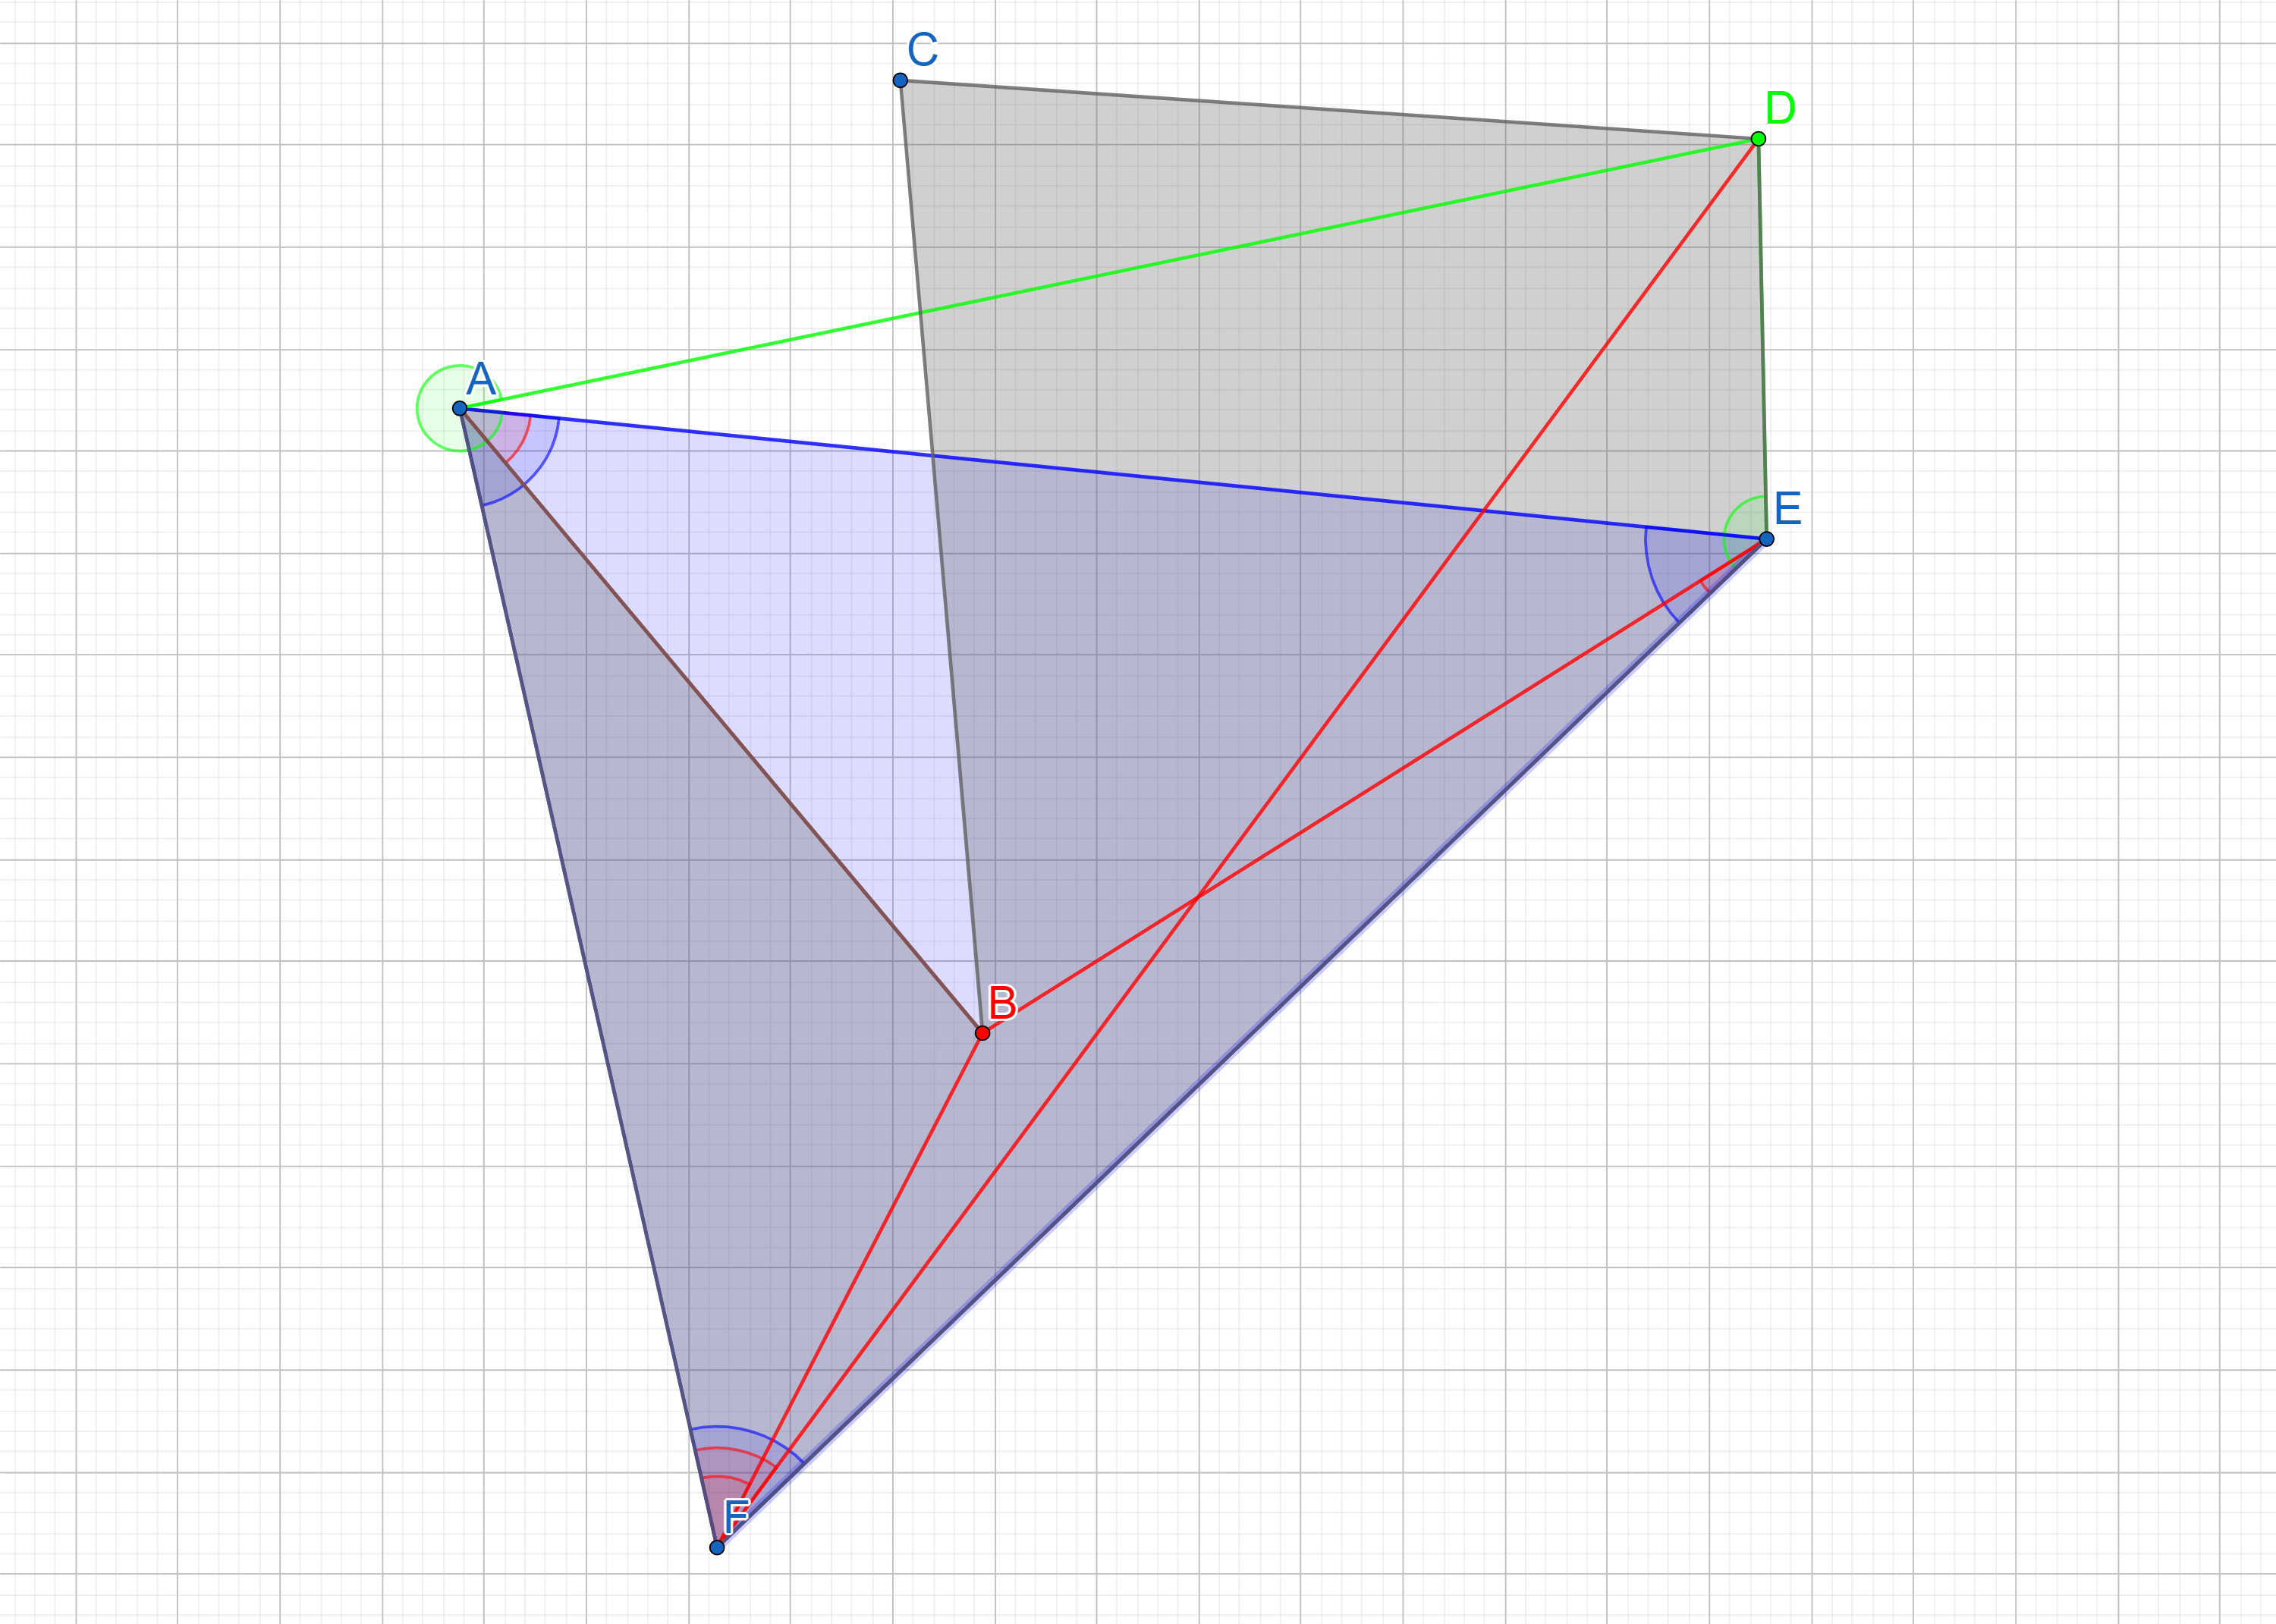
\includegraphics[width=\textwidth]{polygon-with-triangle}
    \caption[Příklad hledání ucha v šestiúhelníku]{
    Příklad hledání ucha v šestiúhelníku ABCDEF}
    \small\emph{
    U trojúhelníku AEF se postupně zkouší ostatní body, zda se nacházejí uvnitř. K bodu D má alespoň jeden z vrcholů vektor s větším úhlem než je úhel ramen -- bod D se nachází mimo a trojúhelník AEF stále může být ucho. K bodu B mají všechny vektory od vrcholů trojúhelníku menší úhel, než je úhel ramen, jedná se tudíž o bod uvnitř a trojúhelník AEF nemůže být ucho.}
\end{figure}

Funkce \texttt{triangulate} nejprve všechny vrcholy stěny přepíše do oboustranného spojového seznamu (\texttt{list}); společně s jejich polohou se uloží také jejich číslo udávající pořadí vrcholu na obvodu mnohoúhelníka. Poté jsou odstraněny všechny duplikáty v seznamu (duplikát se rozpozná podle stejné polohy a odlišného pořadového čísla). Do kontejneru typu \texttt{vector} (nazývá se \texttt{map}) jsou zapisována jednotlivá ucha s použitím pořadových čísel vrcholů. Podle těchto pořadových čísel se nakonec ze seznamu vrcholů vyberou ty správné. Pro výpočet orientovaných úhlů ve stěně, jež jsou později použity pro kontrolu uch, musí aplikace mít referenční vektor každé stěny (jako referenční zde slouží normálový vektor, který je spočítán a později také znovu využit, pokud ho již čtený soubor neobsahoval). Samotné dělení na trojúhelníky pak probíhá tím způsobem, že se postupně kontroluje každý trojúhelník tvořený třemi po sobě jdoucími body, zda v sobě obsahuje některý ze zbývajících vrcholů. U každého vrcholu, který není součástí kontrolovaného trojúhelníku, se spočítá úhel (vektoru od vrcholu trojúhelníku ke kontrolovanému bodu) k rameni trojúhelníku\footnote{Ramena jsou dvě a tím pádem i úhly jsou dva -- vždy je brán v potaz ten větší.}. Pokud je tento úhel větší než úhel mezi rameny, nachází se kontrolovaný bod určitě mimo potenciální ucho a můžeme podobným způsobem testovat další body. V opačném případě si ještě nemůžeme být jisti, že vrchol leží uvnitř, takže se musí otestovat všechny vrcholy ucha vůči tomuto bodu analogicky. Pokud jsou všechny body mimo testované ucho, pořadová čísla bodů se zaznamenají do kontejneru \texttt{map} a prostřední bod ucha se odstraní ze spojového seznamu. Tímto způsobem se postupuje dokud ze strany nezbyde trojúhelník. Nakonec se původní \texttt{vector} s uspořádanými trojicemi upraví podle \texttt{map} a rozdělení je hotové.

\subsection{Metoda \texttt{render}}
Tato funkce zajišťuje vykreslování všech objektů ve scéně. Ze všeho nejdříve je původní snímek přemazán novou barvou pozadí a vyčistí se buffer zaznamenávající barvy a také buffer pro test hloubky. Potom se zvolí shader program, který jsme si v konstruktoru připravili -- sdělíme grafické kartě způsob, jak má data zpracovávat. Protože chceme, aby se v každém snímku kamera mohla posouvat, zavoláme její funkci \texttt{move}. Dále nastavíme tzv. uniform\footnote{\label{uniform}Uniform je zvláštní druh proměnných, ke kterému mají přístup všechny shadery v použitém shader programu. Mohou to být matice, vektory nebo jen jednotlivá čísla.} transformační matice\footnote{Vysvětlení transformačních matic viz \ref{kamera}} pro výpočet pozice bodů ve scéně a uniform\cref{uniform} vektory (o pozici světla a jeho barvě) pro výpočet barvy s osvětlením. Samotné vykreslování je provedeno zavoláním metody \texttt{draw} u všech objektů, které mají uloženou hodnotu \emph{true} v členu \texttt{show}. Nakonec hlavní vlákno programu počká, než grafická karta vše vykreslí.

Tento přístup, kdy každý objekt zvlášť volá vykreslování pro svoje body, má na jednu stranu výhodu v jednoduchosti, na druhou stranu je ale poměrně neefektivní. Existují způsoby, jak celou scénu vykreslit v jednom volání -- o to jsem se pokusil, ale narazil jsem na problémy v shaderech, které se mi nepodařilo vyřešit, takže je implementován tento jednodušší způsob (kdy každý objekt se vykresluje zvlášť). Jde ale spíše jen o teoreticky špatnou optimalizaci, protože v realitě jsem se při vykreslování i poměrně složitých objektů nikdy nedostal do situace, kdy by snímky klesly pod frekvenci monitoru.

\section{Třída \texttt{VertexArray}}
Všechna data, která chceme grafické kartě přes knihovnu OpenGL poskytnout, se musí posílat přes tzv. buffery. Většina bufferů je vymyšlena pro nějaký konkrétní účel kvůli svým vlastnostem (například limitu velikosti, datovému typu), ale jsou i buffery bez přesného určení a záleží na vývojáři, zda je použije. Buffery ale samy o sobě nelze k vykreslování použít -- musí se spojit v tzv. vertex array (tato třída je určena právě pro správu objektu vertex array). Ve vertex array může být od každého typu bufferu vždy jen jeden, protože každý buffer, který by měl být použit, musí být nejdřív aplikován\footnote{Některé struktury knihovny OpenGL nelze používat přímo (např. pomocí ukazatele nebo identifikačního čísla), ale je nutno je \uvoz{aplikovat}. Pokud si kupříkladu chceme zvolit, jaký buffer nebo texturu použít. Funkce pracující s těmito strukturami vždy použijí aktuálně aplikovanou strukturu konkrétního typu -- např. pokud funkce vykreslování chce použít 2D texturu, použije jen tu aplikovanou 2D texturu. Tento proces aplikování se nazývá \emph{binding}.}; od každého typu objektu je vždy aplikovaný jen jeden.

\subsection{Spojení bufferů a třída \texttt{VertexBuffer}}
Tato třída byla navržena tak, že by mohla držet více různých bufferů; buffery jsou se svým vertex array spojeny metodou \texttt{link}, která je uloží do kontejneru \texttt{vector}. V tomto kontejneru se nacházejí uložená identifikační čísla a typy bufferů. Za současné situace je ale použit pouze jeden typ, a to vertex buffer -- ten je v této aplikaci vytvořen a spravován třídou \texttt{VertexBuffer}. Třída \texttt{VertexBuffer} jen drží identifikační číslo vertex bufferu a zvlášť ještě data, která do něj byla vložena, aby bylo umožněno instanci třídy zkopírovat a znovu vytvořit nový buffer. Data jsou do třídy \texttt{VertexBuffer} dodávána metodou \texttt{sendData}\footnote{Při vložení dat do bufferu, v němž již data uložená jsou, dochází ke smazání všech původních dat.}.

Když jsou všechny buffery, jež máme v plánu využít (v našem případě vždy jen jeden), připojeny metodou \texttt{link} a chceme již vertex array začít používat, musíme ještě OpenGL oznámit, jak má data z bufferů pro shadery interpretovat. To má za úkol metoda \texttt{enable}, která OpenGL informuje o tom, jak má všechna data rozdělovat do proměnných u každého volání shaderu. V této aplikaci je pro každý bod 11 čísel: první tři jsou souřadnice v prostoru; pak následují čísla udávající barvu\footnote{Barva je vyjádřena desetinnými čísly (od 0 do 1) v pořadí RGB -- 1. udává červenou barvu, 2. zelenou a 3. modrou. Také lze barvu udávat ke každému bodu objektu zvlášť -- tato možnost není ale v aplikaci implementovaná.}; dále jsou dvojrozměrné souřadnice textury a nakonec trojrozměrné souřadnice normálového vektoru. Celkově z dat tedy shader dostane ke každému bodu tři trojrozměrné a jeden dvojrozměrný vektor -- všechny v sobě mají čísla s plovoucí řadovou čárkou.

\section{\label{objekt}Třída \texttt{Object}}
Každý objekt ve scéně je zvláštní instancí této třídy -- všechny instance jsou drženy v kontejneru \texttt{vector} třídou GraphicsManager. Každý objekt v sobě obsahuje všechny informace o sobě -- jako např. jméno, ukazatel na třídu své textury\footnote{Pokud objekt žádnou texturu nemá, drží nulový ukazatel.} (\texttt{Texture}), polohu a rotaci vůči středu scény.

\subsection{Vytvoření nového objektu}
Když je načten celý soubor a data z něj zpracována do čtyř kontejnerů \texttt{vector}, zbývá všechna tato data spojit a načíst je do vertex bufferu a následně vertex array. Finální tvar, z něhož se data načtou do bufferu, je pole čísel s plovoucí řádovou čárkou -- je tedy potřeba všechny kontejnery s daty spojit do jednoho pole. To se týká i dat o čárách, které nejen že jsou udávány po dvou místo po třech bodech, ale také v souboru nemohou mít žádné informace o souřadnicích textury a normálových vektorech. Tyto chybějící informace jsou doplněny nulami; to se ostatně týká i trojúhelníků, u nichž tyto informace v souboru chyběly (u nich se ale takto doplní jen souřadnice textury, protože normály jsou již dopočítány metodou \texttt{triangulate} třídy \texttt{GraphicsManager}). Čáry se ukládají za data o trojúhelnících a je zachován jejich počet v proměnné.

\subsection{Metoda \texttt{draw}}
Důležitou částí celého procesu vykreslování je metoda \texttt{draw}. S použitím této metody se každý objekt zvlášť vykreslí na scénu.

Než můžeme objekt vykreslit, musíme aplikovat správnou texturu. Nejprve proto zjistíme, zda vůbec objekt texturu má -- kontrolujeme ukazatel na třídu \texttt{Texture} (pokud je nulový, objekt žádnou texturu nemá). Pokud objekt texturu má, jsou o tom shadery informovány uniform\cref{uniform} proměnnou\footnote{Proč potřebujeme shadery explicitně informovat, je vysvětleno v kapitole o třídě \texttt{ShaderManager}} a textura je aplikována pomocí \emph{bindingu}. Poté se vypočítá transformační matice\footnote{Vysvětlení transformačních matic viz \ref{kamera}} pro posun a rotaci objektu vůči středu scény a aplikuje správný režim vykreslování trojúhelníků\footnote{O režimech zobrazování trojúhelníků viz \ref{panel}}. Stejně jako texturu musíme ještě aplikovat vertex array se všemi daty o bodech objektu a nakonec zbývá už zavolat samotné vykreslení -- je provedeno ve dvou voláních (trojúhelníky a čáry se vykreslují zvlášť). Podle počtu čar drženého v proměnné se určí, jak dlouhá část na konci bufferu již nejsou trojúhelníky, ale čáry.

\section{Třída \texttt{Texture}}
Aby bylo možné objekty vykreslovat s texturami, musíme obrázky načíst do speciálního objektu textury a potom tyto objekty v době renderování aplikovat. Tato třída je určena k vytvoření objektu textury z nezpracovaných dat\footnote{Nezpracovanými daty jsou myšlena data o barvě každého pixelu zvlášť.} obrázku, jeho správě (aplikování metodou \texttt{bind}) a smazání. Nezpracovaná data jsou z načtených souborů (různých formátů) získána pomocí knihovny wxWidgets už při načtení těchto souborů. 

Při vytvoření nové textury nastavíme parametry, jak mají shadery vypočítat barvy z jejího obrázku a přiřazovat je k objektu. Když vykreslujeme objekty s texturami, téměř nikdy se nestane, že by textura na obrazovce byla stejně veliká jako originální obrázek a OpenGL musí vědět, jak má s texturou v těchto případech pracovat. Nastavíme zvlášť, jak se má vypočítat výsledná barva textury při zmenšování a zvětšování textury vůči originálu. V obou případech použijeme tzv. bilineární filtrování -- barva se namíchá ve stejném poměru, v jakém je vykreslovaný bod vzdálený od středů čtyř nejbližších pixelů textury. Bilineární filtrování vede k vyhlazenějšímu obrazu bez ostrých hran v texturách. Dále můžeme zvolit tzv. bodové filtrování -- barva se zvolí podle pixelu, k jehož středu má vykreslovaný bod nejblíže. Bodové filtrování je početně méně náročné, ale na druhou stranu výsledný obraz většinou vypadá hůře.

\begin{figure}[h]
    \centering
    \subfloat[\centering Bilineární filtrování]{{
\includegraphics[width=5cm]{filter_linear}}}
    \qquad
    \subfloat[\centering Bodové filtrování]{{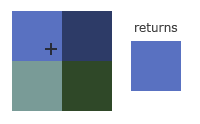
\includegraphics[width=5cm]{filter_nearest}}}
    \caption[Porovnání bodově a bilineárně zfiltrovaného pixelu]{Porovnání bilineárně a bodově zfiltrovaného pixelu~\cite{pic:colorfilter}}
\end{figure}
\begin{figure}[H]
    \centering
    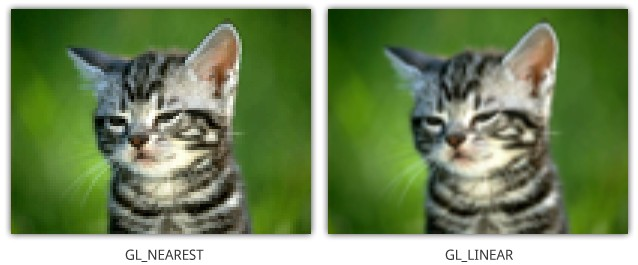
\includegraphics[width=12cm]{texture-comparison}
    \caption[Porovnání bodově a bilineárně zfiltrované textury]{Porovnání bodově a bilineárně zfiltrované textury~\cite{pic:texfilter}}
\end{figure}

Dále pro operaci zmenšování vůči originálnímu obrázku textury využijeme tzv. mipmapy. Při načtení textury se z originálního obrázku vytvoří několik kopií se zmenšeným\footnote{U zmenšení lze zvolit způsob, jakým má být provedeno; zde je použito opět bilineární filtrování.} rozlišením. Když je vykreslovaná stěna s texturou ve scéně menší než textura původní, vymění OpenGL automaticky texturu za její variantu s menším rozlišením\footnote{Nemusí jít vždy o ostrou výměnu, ale častěji spíše o výpočet průměru mezi dvěma nejbližšími velikostmi textury. Způsob, jakým se použije mipmapa, lze vybrat; zde v aplikaci je použita metoda s průměrem, která se také nazývá trilineární filtrování.}; objekt vypadá lépe a ještě se tím ušetří paměť grafické karty.

\begin{figure}[h]
    \centering
    \subfloat[\centering Hotová mipmapa~\cite{pic:mipmap}]{{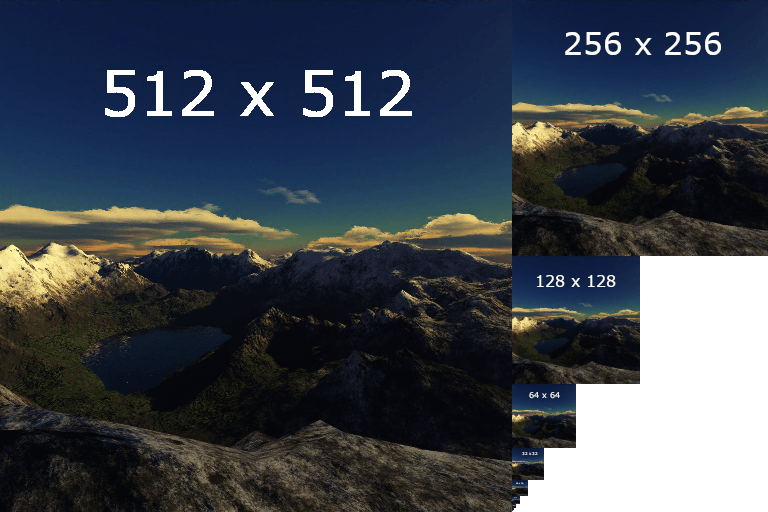
\includegraphics[width=0.4\textwidth]{mipmap}}}
    \qquad
    \subfloat[\centering Jak mipmapa změní výsledný obraz~\cite{pic:mipmap-comparison}]{{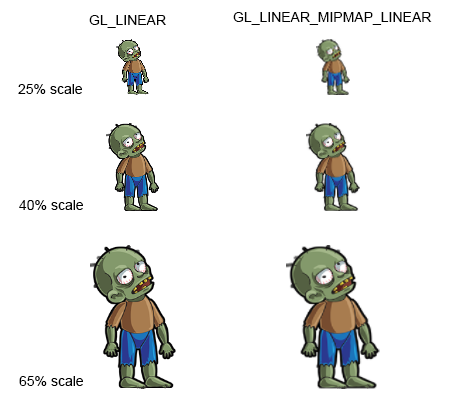
\includegraphics[width=0.5\textwidth]{mipmap-comparison}}}
    \caption{Mipmapa a její použití}
\end{figure}

Po nastavení výše popsaných parametrů jsou nahrána data obrázku a vytvořena mipmapa. Nyní už lze texturu normálně používat.

\section{\label{kamera}Třída \texttt{Camera}}
Úkolem třídy \texttt{Camera} je výpočet transformačních matic, pomocí kterých může potom vertex shader zjistit, kam má jednotlivé body umístit. Tato třída také zpracovává data o myši (tlačítka a pohyb) pro změnu polohy kamery (data jsou poskytnuta třídou \texttt{Canvas}.

\subsection{Transformační matice}
Transformačními maticemi je manipulováno se všemi body ve scéně, aby se vyrenderovaly na místě, kde by měly být. OpenGL žádný objekt kamery, u nějž by jen stačilo volat funkci pohybu nebo rotace, nemá. Stejně tak i souřadnice objektu ve scéně a perspektiva -- to všechno musí být vyřešeno až samotnou aplikací. OpenGL dává k dispozici jen vykreslit trojúhelníky, čáry a body s trojrozměrnými\footnote{Ve skutečnosti jsou použity souřadnice čtyřrozměrné -- detaily níže v textu.} souřadnicemi; jsou použity tzv. normalizované souřadnice\footnote{Při použití normalizovaných souřadnic se neudává počet pixelů, ale relativní pozice vůči velikosti viewportu -- v případě OpenGL používáme souřadnice od -1 do +1 (bod [0,0] je střed, -1 je levý a spodní kraj a +1 je pravý a horní kraj viewportu).} (normalized device coordinates; obr. \ref{normalized}). 

\begin{figure}[h]
	\centering
    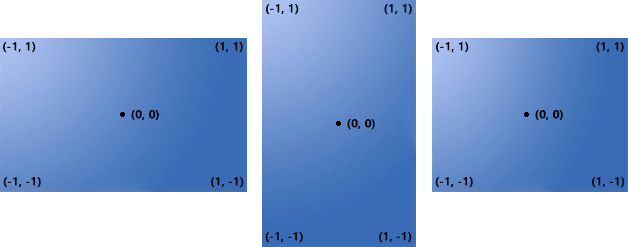
\includegraphics[width=12cm]{normalized-coordinates}
    \caption[Normalizované souřadnice]{\label{normalized}Normalizované souřadnice různých viewportů~\cite{pic:normalized-coordinates}}
\end{figure}

Principem transformačních matic je, že pokud vynásobíme vektor od počátku k bodu objektu jednotkovou maticí\footnote{Jednotková matice je v 3D aplikacích čtyřrozměrná matice. Vynásobíme-li s ní vstupní vektor, bude výsledný vektor stejný jako vektor na začátku.}, v níž se specifickými hodnotami manipuluje, můžeme bod v prostoru posunout nebo otočit. Obecné transformační matice pro posun a změnu velikosti jsou poměrně jednoduché, ale obecná matice pro rotaci v prostoru využívá kvaterniony (rozšíření oboru komplexních čísel určené právě pro řešení rotací v prostoru~\cite{wiki:kvaterniony}). Avšak díky knihovně GLM lze všechny tyto operace provést poměrně jednoduše -- stačí vytvořit jednotkovou matici\footnote{Vytvoření jednotkové matice, stejně jako všechny běžné operace s maticemi jsou součástí knihovny GLM.}, na níž aplikujeme příslušné funkce.

\begin{figure}[h]
    \begin{minipage}{0.45\textwidth}
        \[
        \begin{bmatrix}
            a&0&0&0\\
            0&b&0&0\\
            0&0&c&0\\
            0&0&0&1
        \end{bmatrix}
        \cdot
        \begin{pmatrix}
            x\\
            y\\
            z\\
            w\\
        \end{pmatrix}
        =
        \begin{pmatrix}
            a \cdot x\\
            b \cdot y\\
            c \cdot z\\
            w\\
        \end{pmatrix}
        \]
        \centering
        \small Obecná matice pro změnu velikosti
    \end{minipage}
    \qquad
    \begin{minipage}{0.45\textwidth}
        \[
        \begin{bmatrix}
            1&0&0&a\\
            0&1&0&b\\
            0&0&1&c\\
            0&0&0&1
        \end{bmatrix}
        \cdot
        \begin{pmatrix}
            x\\
            y\\
            z\\
            1\\
        \end{pmatrix}
        =
        \begin{pmatrix}
            x + a\\
            y + b\\
            z + c\\
            1\\
        \end{pmatrix}
        \]
        \centering
        \small Obecná matice pro posun
    \end{minipage}
    \caption{Příklady transformačních matic pro 3D prostor}
    \small\emph{
    Obecná matice má v sobě vyměněnu hodnotu w za číslo 1, protože v době, kdy se tento vzorec aplikuje, vždy platí \(w=1\) (a s jinými hodnotami by translace takto nefungovala); w se mění až při výpočtu perspektivy, který se z tohoto důvodu provádí vždy až jako poslední.
    }
\end{figure}

Přesto, že body umísťujeme do trojrozměrného prostoru, počítáme s jejich polohou vůči počátečnímu bodu vždy jako s čtyřrozměrným vektorem -- čtvrtá hodnota (bývá označována písmenem \emph{w}) je na začátku výpočtů nastavená na 1. Tato poslední hodnota se před vyrenderováním bodu odstraní a všechny ostatní souřadnice vektoru jsou jí vyděleny (tuto poslední fázi s vydělením udělá OpenGL samo). Hodnota \emph{w} se používá pro znázornění perspektivy, kdy čím dál se bod od kamery nachází, tím na vyšší číslo je nastavena.

\begin{minipage}{\textwidth}
Pro získání výsledné polohy všech bodů používá aplikace tři různé transformační matice:
\begin{itemize}
    \item \textbf{model} -- vypočítána samotným objektem v metodě \texttt{draw}; cílem je přesunout a otočit objekt vůči středu scény na své místo
    \item \textbf{view} -- vypočítána v metodě \texttt{viewMatrix}; je použita pro posun všech bodů podle pozice kamery (ve scéně se nám zdá, že pohybujeme kamerou, ve skutečnosti však pohybujeme všemi body a kamera je stále stejná)
    \item \textbf{projection} -- vypočítána pomocí GLM; podle vzdálenosti bodů od kamery a zorného pole upravuje jejich hodnotu \emph{w}, aby obraz získal perspektivu; kromě té ale ještě posune všechny body mimo specifikovanou vzdálenost pryč ze scény, takže je OpenGL nevyrenderuje -- pokud jsme od nějakých bodů moc daleko nebo naopak moc blízko, jsou odstraněny
\end{itemize}
\end{minipage}

\subsection{Metoda \texttt{viewMatrix}}
Tato metoda vrací matici \emph{view}; ta je spočítána s pomocí funkce \texttt{lookAt} (z knihovny GLM) procesem tzv. Gram–Schmidtovy ortogonalizace~\cite{libre:ortogonalizace}. Díky ní získá GLM bázi souřadnic kamery z vektoru od středu rotace\footnote{\label{rotace}Středem rotace je myšlen bod, okolo kterého kamera rotuje.} ke kameře, vektoru od středu scény ke středu rotace a vektoru směrem vzhůru. Při zavolání funkce je nejprve zajištěno, aby se kamera nemohla točit a přibližovat donekonečna, protože potom by výpočty vektoru od středu rotace ke kameře přestaly fungovat správně. Následuje výpočet tohoto vektoru\footnote{Ve skutečnosti probíhá výpočet vektoru z opačného směru (počítá se vektor od kamery k středu rotace), který je nakonec odečten při volání funkce \texttt{lookAt}.} vycházející z dat o rotaci kamery. Před voláním funkce \texttt{lookAt} je ještě spočítán posun středu rotace. Když jsou všechny vektory připraveny, můžeme nechat GLM vytvořit samotnou matici.

\subsection{Metoda \texttt{move}}
Aby mohla metoda \texttt{viewMatrix} vytvářet různé matice, musí se měnit vlastnosti kamery -- pozice a rotace. Metoda \texttt{move} mění v závislosti na myši právě tyto vlastnosti kamery. Zvlášť je vyhodnocena rotace a zvlášť změna pozice, protože každý z těchto pohybů uživatel ovládá jinou interakcí s myší\footnote{Konkrétní informace o ovládání viz \ref{ovladaniKamery}}. Vždy je zkontrolováno, zda uživatel minulý snímek již tlačítko držel stisknuté -- kromě zoomu (přibližování a oddalování), kde kolečko uživatel držet stisknuté nemusí. Pokud ano, zjistí se rozdíl mezi pozicí myši v minulém a současném snímku; rozdíl je vynásoben citlivostí rotace nebo pohybu a přičten k příslušnému pohybu. Pokud ne, pouze se v proměnné zaznamená, že uživatel v tomto snímku držel tlačítko.

\section{\label{shadery}Shadery a třída \texttt{ShaderManager}}
Shadery jsou programy určené pro grafickou kartu počítače. Jsou jim posílána data o poloze a barvách bodů, textury; jejich cílem je z těchto dat vypočítat, jakou barvu by měly mít jednotlivé pixely zobrazené uživateli (ve většině případů\footnote{Ne každý shader musí mít za cíl něco uživateli zobrazit; např. compute shadery většinou nic nevykreslují. Také data posílaná shaderům nejsou předem určena, ale informace o bodech jsou data, která se do shaderů posílají nejčastěji.}). Shaderů je více druhů -- např. vertex, fragment, geometry, compute. Každý druh má svoji specifickou roli a spojují se dohromady do tzv. shader programu. V shader programu může být více shaderů stejného druhu, ale také od některých druhů nemusí být shader použit žádný -- záleží na účelu daného programu. Podle druhů (kvůli neměnnému fungování grafického řetězce je pevně dáno, v jakém pořadí k datům různé druhy shaderů přistupují) a pořadí připojení shaderů do shader programu se určí, v jakém sledu budou data shadery procházet. Na tom záleží, protože pokud první shader dostane z vertex array data, jež sám nepoužije, musí být nastaveno, aby byla data v řetězci poslána dále (až k shaderu, který je využije). V této aplikaci grafická karta používá jeden shader program s dvěma shadery; jeden je druhu vertex a druhý fragment.

Protože je větší množství grafických karet (i od různých výrobců) s různými architekturami, jsou shadery vždy kompilovány při spuštění programu -- z toho důvodu jsou součástí jinak plně postavené aplikace také zdrojové kódy.

\subsection{Vertex shader}
První shader v grafickém řetězci je vertex shader, který má za úkol u každého vrcholu určit, kde leží. Proto vždy musí nakonec některý z vertex shaderů (v této aplikaci je pouze jeden) napsat výslednou polohu bodu do proměnné \emph{gl\_Position}\footnote{V shaderech se někde vyskytují předdefinované proměnné -- vždy začínají sekvencí \emph{gl\_}...}. Vertex shader je v této aplikaci obsažen v souboru \emph{default.vert}. Výslednou pozici bodu získá rozšířením jeho trojrozměrných souřadnic, které získal z vertex array, na čtyřrozměrný vektor (kde \(w=1\)), jejž vynásobí postupně se všemi transformačními maticemi\footnote{Transformační matice nejsou uloženy ve vertex array, protože se mohou každým snímkem měnit -- posílají se do shaderů jako uniform\cref{uniform} proměnné.}.

Všechna data z vertex array se posílají dále do fragment shaderu, protože se s jejich pomocí bude počítat barva (poloha bodů je potřeba také, protože se použije při výpočtu osvětlení). Barva bodu a souřadnice textury jsou odeslány beze změn, ale normálové vektory a poloha bodu musí být upravena. Poloha bodu by měla odpovídat skutečné poloze ve scéně, takže musí být vynásobena transformační maticí \emph{model}. Normálové vektory jsou upraveny, aby je nerozhodilo, pokud by se objektu změnil poměr stran (k tomu zatím nikdy v této aplikaci nedochází, ale je to příprava, pokud by to v budoucnu bylo umožněno.)

\subsection{Fragment shader}
Po vertex shaderu přichází na řadu fragment shader, kde jsou nastaveny barvy všech zobrazených pixelů. Fragment shader je pro tuto aplikaci uložen v souboru \emph{default.frag}. Výsledná barva je odeslána ve formě vektoru dál a OpenGL ji poté zobrazí uživateli. Fragment shader počítá, jak by měly různé strany být osvětleny podle úhlu na ně dopadajícího světla. Nejprve zkontroluje, zda vůbec normálový vektor použitý na výpočet osvětlení někam směřuje; pokud ne, jde o čáru (bez textury) a rovnou může být vrácena barva povrchu bez úprav. Pokud se jedná o stěnu, může být spočítáno osvětlení.

Světlo v počítačové grafice (obzvlášť v aplikacích, jež se mají renderovat v reálném čase) je vždy kompromis mezi realističností a složitosti výpočtu. V této aplikaci se používá relativně jednoduchý model osvětlení; konkrétně kombinace tzv. ambientního a rozptýleného (difúzního) osvětlení. Při použití ambientního osvětlení předpokládáme, že ať se ve scéně nacházíme kdekoliv vůči zdroji světla, vidíme vždy alespoň trochu. S ambientním osvětlením se tedy nikdy nemůže stát, že by objekt neměl žádnou barvu, protože by byla příliš velká tma. Difúzní osvětlení jsou paprsky z určitého směru -- i když světlo může pocházet z bezrozměrného bodu, bude se vždy chovat jako světlo s rovnoběžnými paprsky z tohoto směru. Síla ambientního světla je na každou stěnu konstantní. Síla rozptýleného světla na stěnu se ve fragment shaderu vypočítá jako absolutní hodnota z kosinu úhlu normálového vektoru strany a vektoru od světla k bodu strany. Celkové světlo se spočítá tak, že je síla obou světel vynásobena příslušným koeficientem,\footnote{Koeficienty je globálně ovlivněna síla konkrétního druhu světla.} barvou světla (v případě této aplikace se nic nezmění, protože světlo má bílou barvu) a nakonec jsou obě světla sečtena.

Nakonec už zbývá jen vynásobit celkové světlo s barvou objektu nebo textury (pokud jí objekt disponuje -- to fragment shader zjistí uniform proměnnou).

\subsection{Třída \texttt{ShaderManager}}
Třída \texttt{ShaderManager} v sobě drží kontejnery \texttt{vector} s chytrými ukazateli (konkrétně \texttt{unique\_ptr}) na objekty třídy \texttt{Shader}. Každá instance třídy \texttt{Shader} při vytvoření načte specifikovaný soubor a pokusí se ho zkompilovat -- nová instance vznikne při každém volání metody \texttt{addShader} třídy \texttt{ShaderManager}.

Když jsou všechny potřebné shadery načteny, je shader program vytvořen metodou \texttt{linkProgram}. Pokud kompilace u kteréhokoliv shaderu selhala, aplikace se ukončí s chybovou hláškou; při postavení aplikace v režimu ladění se ještě do terminálu vypíše, proč k selhání došlo. Abychom vytvořený shader program použili při vykreslování, musíme zavolat ještě metodu \texttt{useProgram}.

\chapter{Programovací prostředky}
\section{Programovací jazyk}
Téměř celý program byl vytvořen v jazyce C++, který jsem si zvolil proto, že byl se dal celkově popsat jako plně vybavený; má všechny možnosti objektového programování zároveň s nízkoúrovňovými možnostmi jazyka C. Podle statistik vyhledávání na stránkách společnosti Google se jedná o pátý nejpoužívanější programovací jazyk na světě~\cite{github:pypl}. Není interpretovaný, takže nabízí vysoký výkon proti všem interpretovaným jazykům (jako je z populárních jazyků např. Python).

Shadery jsou napsané v jazyce GLSL (OpenGL shading language), což je speciální jazyk právě pro psaní shaderů pro knihovnu OpenGL. Místo GLSL lze zvolit několik alternativ, ale ty nejsou tak časté (bude složitější pro ně najít podporu v případě problémů) a mívají problémy s kompatibilitou.

\section{Knihovny}
Pro projekt jsem využíval několik knihoven. Knihovnu wxWidgets jsem použil pro grafické ovládání aplikace a načítání obrázků textur. OpenGL bylo použito na prostorové zobrazování -- zprostředkuje v programu komunikaci s ovladačem grafické karty počítače. Ve spojení s OpenGL použil knihovnu GLM (OpenGL Mathematics), jež přidává nové datové typy (vektoru a matice) a operace s nimi. Tyto nové datové typy fungují stejně jako v GLSL a lze je do shaderů posílat přímo. Kromě GLM ještě k OpenGL používám knihovnu GLEW, která mi poskytne ukazatele na funkce a konstanty OpenGL.

\chapter{Instalace}
V odkazu ke stažení jsou k dispozici tři ZIP archivy:
\begin{itemize}
    \item \textbf{release.zip} -- předem postavený program se všemi potřebnými soubory
    \item \textbf{build.zip} -- program připravený k sestavení (všechny knihovny mají soubory již rozdělené do souborové struktury)
    \item \textbf{samples.zip} -- testovací objekty a textury k některým z nich
\end{itemize}

Archiv \emph{release.zip} stačí pouze dekomprimovat a program je poté plně funkční. Je možné stáhnout kořenovou složku projektu, soubory knihoven stáhnout, rozdělit do příslušných složek a program potom postavit. Při použití archivu \emph{build.zip} lze přeskočit stahování a rozdělování souborů knihoven (sekce \ref{libs}) a rovnou aplikaci postavit.

\section{Systémové požadavky}
Aplikace je určena pro 64-bitový operační systém Windows -- byla testována na Windows 10 (sestavení 19042.1586) a Windows 11 (sestavení 22000.556). Velikou roli u aplikací s OpenGL hrají grafické ovladače -- během testování na dvou různých počítačích (s různými grafickými kartami) jsem našel několik situací, v nichž program fungoval jen na jednom z nich. Aplikaci jsem testoval s grafickými kartami \emph{Intel Iris Xe Graphics G7 96} a \emph{Nvidia GTX 1080 Ti}. Přechod mezi grafickými kartami od stejného výrobce většinou nepůsobí problémy, ale přechod mezi grafickými kartami různých výrobců může být horší. Pokud se přechází na grafickou kartu o několik generací starší, je větší šance, že software nebude plně kompatibilní.

\section{Knihovny}
\begin{itemize}
    \item wxWidgets 3.1.5~\cite{lib:wxwidgets}
    \item OpenGL Mathematics (GLM) 0.9.9.8~\cite{lib:glm}
    \item OpenGL Extension Wrangler (GLEW) 2.1.0~\cite{lib:glew}
\end{itemize}
Při použití souborů \emph{release.zip} nebo \emph{build.zip} není třeba žádnou z výše popsaných knihoven stahovat, protože všechny potřebné části jsou již součástí archivu (včetně souborů s licenčními podmínkami\footnote{Licenční podmínky knihoven vyžadují, aby s jakoukoliv jejich distribucí (zdrojový kód nebo binární soubory) byly tyto soubory dodány.} ve složce \emph{licenses}). OpenGL (konkrétně verze 4.6) ale na druhou stranu je potřeba nainstalovat (pokud už není nainstalováno), protože se může s každou grafickou kartou lišit. Z toho důvodu je OpenGL vždy nainstalováno s ovladačem grafické karty -- stačí nainstalovat nebo aktualizovat tento ovladač.

\subsection{\label{libs}Rozdělení do složek}
Tento krok je možné přeskočit, pokud je použit archiv \emph{release.zip} nebo \emph{build.zip}.

K wxWidgets je potřeba stáhnout soubory knihovny pro vývoj\footnote{wxMSW-3.1.5\_gcc810\_x64\_Dev.7z}, vydání\footnote{wxMSW-3.1.5\_gcc810\_x64\_ReleaseDLL.7z}, i hlavičky\footnote{wxWidgets-3.1.5-headers.7z}). Archivy s hlavičkami a se soubory pro vývoj stačí dekomprimovat do kořenové složky s projektem. Soubory pro vydání je třeba dát volně (ne ve složce) do \emph{build}.

Stažený archiv knihovny GLM\footnote{glm-0.9.9.8.zip} v sobě obsahuje složku \emph{glm}, v níž je další složka se stejným jménem. Tuto vnitřní je třeba zkopírovat do \emph{include} v kořenové složce projektu.

Ze staženého archivu knihovny GLEW\footnote{glew-2.1.0-win32} by se měl do složky \emph{build} v kořenové složce projektu zkopírovat soubor \emph{glew32.dll}\footnote{V archivu se nachází zde: \emph{glew-2.1.0\textbackslash bin\textbackslash Release\textbackslash x64}}. Celou složku \emph{include} z archivu je třeba přesunout do kořenové složky projektu. Soubor \emph{glew32.lib}\footnote{V archivu se nachází zde: \emph{glew-2.1.0\textbackslash lib\textbackslash Release\textbackslash x64}} se musí přenést do nové složky \emph{lib\textbackslash glew}.

\section{Sestavení}
Pro postavení aplikace je použit kompilátor MinGW (verze 8.1.0). Celý proces je proveden pomocí tzv. makefile (je použit linuxový typ -- pro postavení je nutno mít nainstalovaný také GNU-make). Aby makefile fungoval, je potřeba u MinGW i GNU-make, aby jejich spustitelné soubory byly obsaženy v systémové proměnné \emph{PATH}.

Pokud jsou všechny potřebné části připraveny, lze aplikaci postavit pomocí terminálu v kořenové složce projektu:\\
\texttt{make}

Také lze aplikaci postavit v ladícím režimu, v němž se s oknem aplikace otevře terminál pro výpis informací nebo popř. chybových hlášek (např. podrobnosti k selhání kompilace shaderů):\\
\texttt{make debug}

\begin{minipage}{\textwidth}
Pokud je program přestavěn z jednoho režimu do druhého, musí se nejprve smazat všechny již vytvořené objektové soubory:\\
\texttt{make clean}
\end{minipage}

\section{Ukázkové objekty}
V archivu \emph{samples.zip} jsou ukázkové objekty. \emph{Cube} je krychle s texturou cihel~\cite{sample:brick} a prázdným souborem obrázku pro test, zda program rozpozná nevalidní soubor textury. \emph{Piggy\_bank}~\cite{sample:piggy} je pro testování texture mappingu a soubor \emph{car.obj}~\cite{sample:car} má za účel otestovat načítání velkého souboru s více komplikovanými objekty.

\chapter{Ovládání}
\section{Základní ovládání}
Všemi menu může uživatel procházet pomocí myši a levého tlačítka myši. Kromě toho lze na průchod menu také použít klávesnici -- stisknutím nebo držením levého tlačítka Alt na klávesnici v kombinaci s písmenem, které je podtržené v názvu položky, již chce zvolit. Mezi položkami v menu nebo tlačítky je možné procházet šipkami a volbu potvrdit mezerníkem nebo tlačítkem Enter.

\section{\label{ovladaniKamery}Kamera}
Kameru může uživatel ovládat pomocí myši. Držením levého tlačítka myši a jejím posouváním se kamera otáčí. Stejným způsobem lze za pomocí pravého tlačítka kamerou posouvat. Točením kolečka myši může uživatel upravit přiblížení kamery.

\section{\label{panel}Postranní panel}
V postranním panelu si může uživatel ze seznamu zvolit objekt, u něhož si přeje upravit vlastnosti. Pokud uživatel žádný objekt v seznamu nezvolí, nastavení nebudou mít žádný účinek. Také lze zvolit zaškrtnutím políčka vedle jména objektu, zda se má odpovídající objekt zobrazit.

Po zvolení objektu může uživatel změnit polohu, rotaci, či velikost daného objektu ve scéně pomocí číselných polí. U posunu nebo rotace jsou nastavení rozděleny do tří polí -- pro manipulaci s objektem podle os v prostoru. Rotace je udávána ve stupních.

\begin{minipage}{\textwidth}
Roletou v nejnižším řádku uživatel může přepnout režim, ve kterém se budou stěny objektu renderovat:
\begin{itemize}
    \item \textbf{Fill} -- Základní režim; stěny jsou vyplněné
    \item \textbf{Line} -- Ze stěn se renderují jen jejich hrany
    \item \textbf{Point} -- Ze stěn se renderují jen jejich vrcholy
\end{itemize}
\end{minipage}

Pro snazší organizaci lze objekty duplikovat, mazat a přejmenovat příslušnými tlačítky. Při stisknutí tlačítka pro přejmenování se otevře nové okno, ve kterém lze upravit jméno objektu v textovém poli -- změny lze potvrdit kromě tlačítka \emph{Ok} i klávesou Enter.

Další možností změn u objektů jsou barvy a textury. Na \textbf{obojí} se při vybrání objektu a stisknutí tlačítka otevře příslušné menu -- textury mají menu velmi podobné seznamu objektů, v němž se žádoucí textura vybere a následně potvrdí tlačítkem; u barev lze nejen vybírat z několika, ale také je přímo mixovat. Ve stejný moment má objekt vždy buď barvu, nebo texturu -- vybráním jednoho se zruší to druhé.

\chapter{Závěr}
Celkově jsem s konečnou fází projektu spokojený, i když jsem na začátku čekal, že stihnu udělat více. Hlavním cílem bylo si vyzkoušet programování v relativně složitém programovacím jazyce; k tomu ještě vytvořit grafické uživatelské rozhraní, které jsem nikdy předtím programovat nezkoušel. Myslím si, že těchto cílů bylo dosaženo plně.

Také jsem nikdy s žádnou z použitých knihoven nikdy předtím nepracoval, takže jsem na začátku své práce pořádně nemohl odhadnout, za jak dlouhou dobu budu schopen jednotlivé části programu vytvořit. Z toho důvodu jsem také strávil relativně dlouhou dobu tvořením pravidelné renderovací smyčky s knihovnou, jež na to není uzpůsobena, v programu, kde ani není pro pravidelné renderování žádné využití. V současné podobě by stačilo, kdyby se nové snímky renderovaly jen v době interakce uživatele s aplikací. Renderovací smyčka by byla nezbytná, až pokud bych do aplikace implementoval animace.

Překvapilo mě, jak matoucí může být práce s OpenGL (i přesto, že se jedná o velmi rozšířenou knihovnu). V podstatě k jakémukoliv cíli vede několik různých cest, u nichž jde velmi těžce dohledat jejich výhody a nevýhody. Nejen, že je OpenGL stále vyvíjeno vlastními vývojáři, ale také je jeho součástí přes 700 rozšíření (které většinou pocházejí od různých společností) s velmi limitovanou dokumentací. Tato dokumentace je také většinou napsána pro vývojáře již zběhlé v programování s OpenGL, takže pro mě byla někdy těžce pochopitelná.

Nakonec jsem ale splnil všechny body v zadání a nyní bych byl schopen podobnou aplikaci vyvinout mnohem rychleji a pravděpodobně i lépe. Mimo to jsem se naučil, jak psát dokumentaci pomocí textového procesoru \LaTeX.

\renewcommand{\bibpreamble}{
This software is based in part on the work of the Independent JPEG Group.}

\begin{flushleft}
    \makeatletter
        \interlinepenalty=10000
        \bibliographystyle{czechiso/czechiso}
        \bibliography{citace.bib}
    \makeatother
\end{flushleft}

\clearpage
{
    \pagestyle{lof}
    \fancypagestyle{plain}[lof]{}
    \listoffigures
    \thispagestyle{lof}
}

\end{document}
